\documentclass[a4paper, 10pt, fleqn]{article}

\usepackage[utf8]{inputenc}
\usepackage[T1]{fontenc}
\usepackage{textcomp}
\usepackage{lmodern}
\usepackage[ngerman]{babel}
\usepackage{tocbibind}
\usepackage{enumerate}
\usepackage{xcolor}
\usepackage{pdfpages}
\usepackage{amsmath}
\usepackage{graphicx}
\usepackage{geometry}
\usepackage{scrpage2}
\usepackage{lastpage}
\usepackage[hyphens]{url}
\usepackage{hyperref}
\usepackage{listings}
\usepackage{float}
\restylefloat{figure}
\lstset{language=[ansi]C++}

\newcommand{\code}[1]{\texttt{#1}}

\renewcommand*{\listoffigures}{%
  \begingroup
  \tocchapter
  \tocfile{\listfigurename}{lof}
  \endgroup
}

\geometry{left=3cm, top=3cm, bottom=3cm, right=2cm}

\hypersetup{
    colorlinks,
    linkcolor=black,
    citecolor=black,
    urlcolor=black
}

\pagestyle{scrheadings}
\ihead{PREN1 Gruppe 39}\ohead{Gesamtkonzept} 
\ifoot{\today} \ofoot{Seite \thepage\ von {\hypersetup{linkcolor=black}\pageref{LastPage}}}

% Einrücken zu Beginn von neuem Absatz unterdrücken
\setlength{\parindent}{0pt}

% Zeilenabstand einstellen
\usepackage{setspace}
\makeatletter
\newcommand{\MSonehalfspacing}{%
  \setstretch{1.44}%  default
  \ifcase \@ptsize \relax % 10pt
    \setstretch {1.448}%
  \or % 11pt
    \setstretch {1.399}%
  \or % 12pt
    \setstretch {1.433}%
  \fi
}
\newcommand{\MSdoublespacing}{%
  \setstretch {1.92}%  default
  \ifcase \@ptsize \relax % 10pt
    \setstretch {1.936}%
  \or % 11pt
    \setstretch {1.866}%
  \or % 12pt
    \setstretch {1.902}%
  \fi
}
\makeatother
\MSonehalfspacing


\begin{document}
% !TEX root = Dokumentation.tex
\begin{titlepage}   

\begin{center}
\textsc{\Large PREN Team 39}\\[0.5cm]

% Title
\newcommand{\HRule}{\rule{\linewidth}{0.5mm}}
\HRule \\[0.4cm]
{ \huge \bfseries GüselStar XXI}\\[0.4cm]
{ \LARGE \bfseries Gesamtkonzept}\\[0.4cm]
\HRule \\[1.5cm]

% Unterer Teil der Seite
{\large Horw, \today}

\begin{figure}[H]%Position festigen
\centering
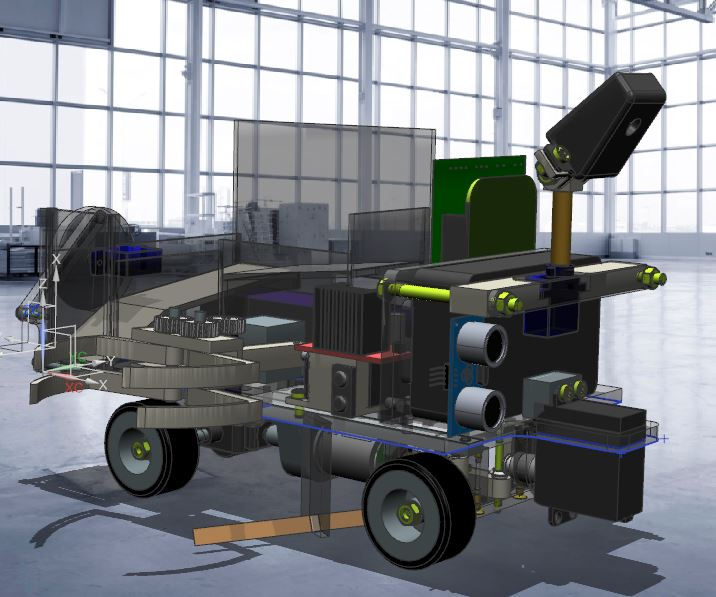
\includegraphics[width=0.7\textwidth]{03_Loesungskonzept/pictures/Tietelbild1.JPG}
\label{fig:activityRoute}
\end{figure}
% Author and supervisor
\begin{minipage}{0.4\textwidth}
\begin{flushleft} \large
\emph{Autoren:}\\
Patrizio Brantschen\\
Stefan Häfliger\\
Tobias Kreienbühl\\
Joël Meloni\\
Silvan Ritz\\
Lars Walther\\
\end{flushleft}
\end{minipage}
\hfill
\begin{minipage}{0.4\textwidth}
\begin{flushright} \large
\emph{Supervisor:} \\
Jürg Habegger
\end{flushright}
\end{minipage}
\large
\vfill
TA.BA\_PREN2.F1601 \\
Hochschule Luzern Technik \& Architektur

\end{center}

\end{titlepage}
\tableofcontents
\clearpage
% !TEX root = ../Dokumentation.tex
\section{Abstract}
Die vorliegende Arbeit befasst sich mit der Konzeptfindung für ein Modell eines autonomen Müllfahrzeuges. Im Rahmen des Moduls Produktentwicklung 1 an der Hochschule Luzern, wird in einer in einer interdisziplinären Zusammenarbeit zwischen Studierenden der Fachrichtungen Informatik, Elektrotechnik und Maschinenbau dieses Konzept erarbeitet. Das Fahrzeug wird im Modul Produktentwicklung 2 hergestellt und muss eine vorgegebene Aufgabe ausführen können. Es wird aufgezeigt wie mehrere mögliche Konzepte entwickelt werden und schlussendlich ein Lösungskonzept zur Herstellung ausgewählt wird. Der Fokus liegt auf Projektmanagement, Budgetplanung, Technologierecherchen, Konzept Erarbeitung, interdisziplinärer Zusammenarbeit und Entscheidungsfindung. Anhand von Tests und Auswertungen wird das Chassis mit 4 Rädern, einer Servomotor angetriebenen Achsschenkellenkung und einem DC-Getriebemotor für den Antrieb bestimmt. Für die Erzeugung der Bilder wird eine drehbare Rasperry-Cam verwendet. Die Bilder für die Fahrbahnerkennung werden mit OpenCV über Raspberry-Pi 2 ausgewertet. Eine weitere Aufgabe des Rapberry-Pi, ist die Informationsverteilung. Für die Kommunikation mit den Hardwarekomponenten wird ein Microkontrollerboard von Freescale eingesetzt. Die genaue Detektierung des zu leerenden Containers erfolgt mittels Infrarotsensoren. Um den Container zu Greifen wird ein Schwenkarm benutzt, welcher mit einem Rundgreifer ausgestattet ist. Das Schüttgut wird über einen Behälter mit abgewinkelten Bodenflächen für das Entladen vorbereitet. Durch das öffnen der Behälterklappe wird das Schüttgut in den Endbehälter entleert.
\clearpage
% !TEX root = ../Dokumentation.tex
\section{Einleitung}
Busfahrer/In und Bus, Lokführer/In und Zug, Chauffeur/In und Auto. All diese Begriffe waren bis vor kurzer Zeit unmittelbar miteinander verbunden. Ohne den jeweils anderen konnte man sich nicht fortbewegen. Doch genau dies ändert sich im Moment. Autonome Fahrzeuge sind längst nicht nur wilde Fantasien, sondern werden von vielen Unternehmen entwickelt. Wenn man auf den Straßen von Kalifornien unterwegs ist, kann es bereits geschehen, dass ein solches autonom fahrendes Auto neben einem an der Ampel steht. Diese Entwicklung ist keineswegs neu, sondern hatte schleichenden Einzug in die Automobil-Branche. Ob mit dem Tempomat oder den automatischen Notbremssystemen, die Grundbausteine wurden bereits in der Vergangenheit gelegt.
Trotzdem ist das autonome Fahren eine ganz neue Herausforderung und erfordert sehr viel neue Technik. Das Potential für solche autonome Fahrzeuge ist riesig. Jedoch sind auch die technischen Anforderungen sehr hoch, damit auch jeder Passagier sicher an sein Ziel kommt und alle Passanten sich sicher bewegen können. \\
Mit genau diesem Problemen ist auch die Aufgabe des Produktentwicklungsmodul 2015/2016 verbunden. Die vorliegende Arbeit soll aufzeigen, wie es möglich sein soll, ein autonomes Entsorgungsfahrzeug zu bauen. Das Entsorgungsfahrzeug muss in der Lange sein auf einem acht förmigen Kurs selbständig zwei Miniatur-Abfallcontainer zu entleeren und das Schüttgut anschliessend auf einer Deponie zu entsorgen.\\
Für das optimale Lösungskonzept wurde die Aufgabenstellung in viele kleine Teilprobleme aufgeteilt. Zu jedem Teilproblem wurden verschiedene Lösungsvarianten gesucht. Die erfolgversprechendsten Varianten wurden näher betrachtet und teilweise mit Funktionsmuster ausgetestet. Diese Arbeit zeigt auf, was die Teilaufgaben sind und welche Lösungen ausgewählt wurden. Weiter ist die Projektstruktur und die Projektplanung aufgeführt. Diese Arbeit beschränkt sich auf die grundlegenden Konzepte. Detaillierte Konzepte oder Implementationen werden Bestandteil von Produktentwicklung 2 sein. 

% !TEX root = ../Dokumentation.tex
\section{Umsetzung}

% !TEX root = ../Dokumentation.tex
\subsection{Gesamtübersicht}

\begin{figure}[h!]%Position festigen
\centering
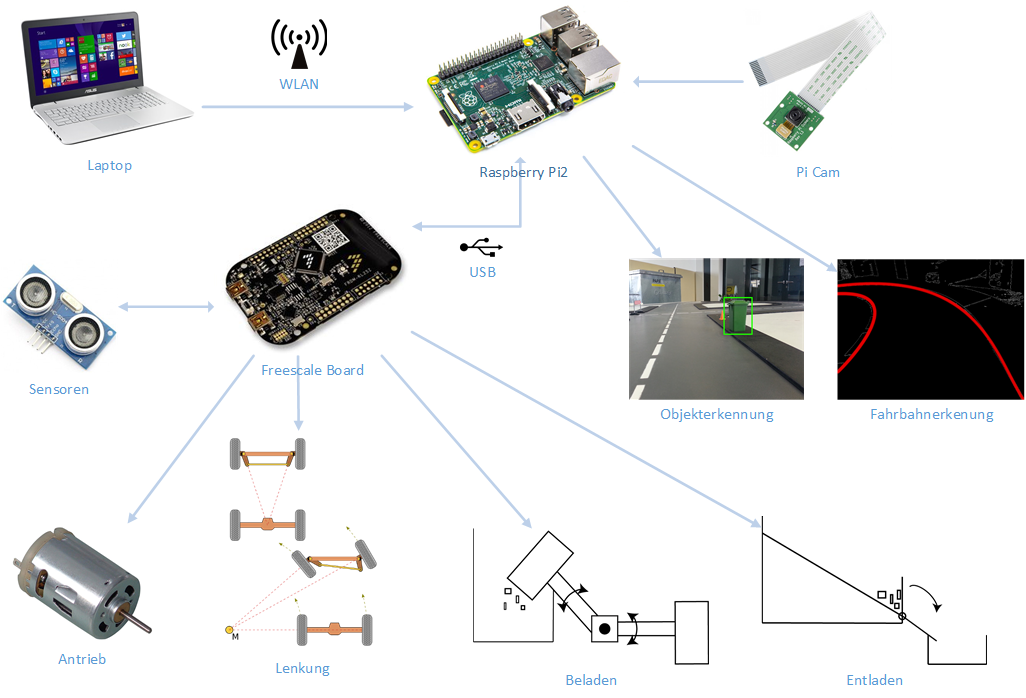
\includegraphics[width=0.9\textwidth]{03_Loesungskonzept/pictures/uebersichtszeichnung.png}
\caption{Übersichtszeichnung}
\label{fig:Java}
\end{figure}

\subsubsection{Zusammenspiel}
\textbf{Funktionsbeschrieb}\\[0.2cm]
Das Herzstück des autonomen Entsorgungsfahrzeug bildet das Microcontrollerboard. 
\textbf{Komponentenbeschrieb}
\textbf{Begründung}
Wenn benötigt
\textbf{Berechnungen}
\textbf{Testergebnisse}

\subsubsection{Schnittstellen}
\textbf{Funktionsbeschrieb}
\textbf{Komponentenbeschrieb}
\textbf{Begründung}
Wenn benötigt
\textbf{Berechnungen}
\textbf{Testergebnisse}
% !TEX root = morphkasten.tex

\section{Chassis}


%############## RAUPEN
\subsection{Raupen}

\begin{figure} [hbp]
	\centering
	\begin{subfigure}[b]{0.4\textwidth}
		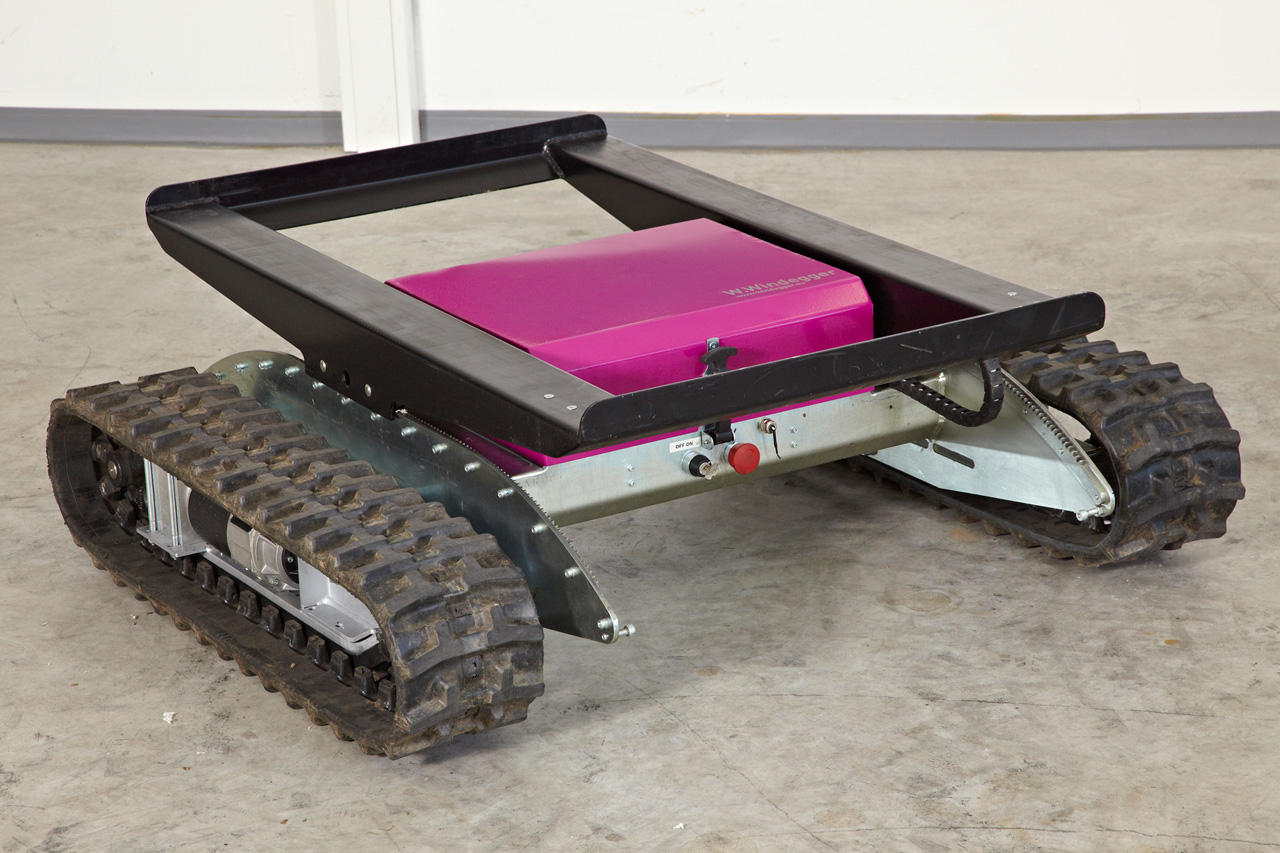
\includegraphics[width=\textwidth]{fig/Raupenfahrzeug.jpg}
		\caption{1. Situation: Modell 
		(Quelle: www.slowine-tech.de)}
	\end{subfigure}
	\hfill
	\begin{subfigure}[b]{0.36\textwidth}
		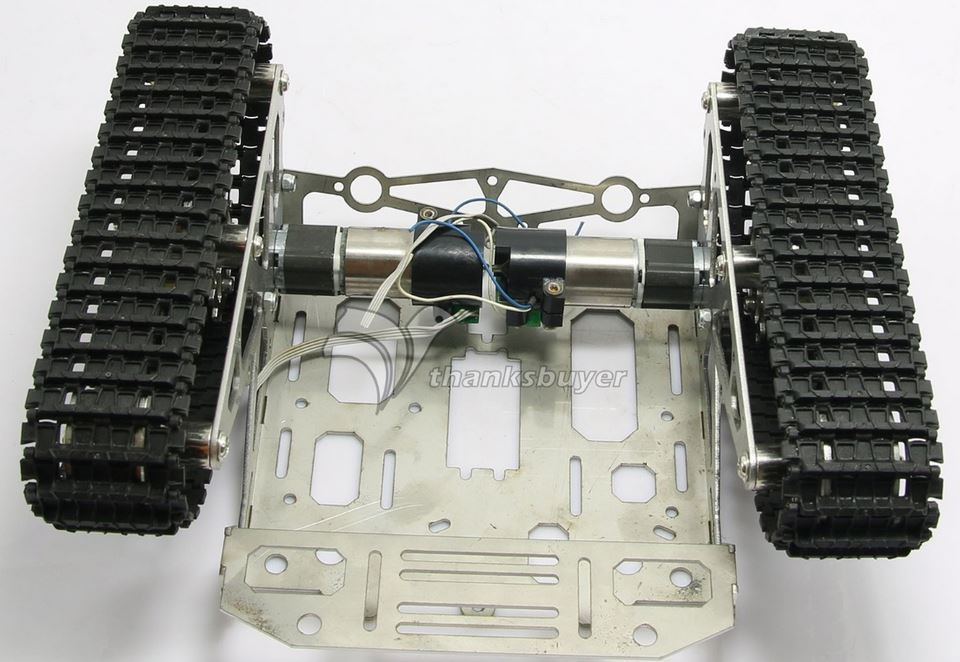
\includegraphics[width=\textwidth]{fig/Raupenfahrzeug-2.JPG}
		\caption{2. Situation: Ansicht von unten
		(Quelle: http://www.sainsmart.com/)}
\end{subfigure}
	\caption{Raupenfahrzeug}\label{fig:animals}
\end{figure}


\begin{table}[h]
\begin{tabular}{p{0.5\textwidth} | p{0.5\textwidth}}


 \textbf{Vorteile} & \textbf{Nachteile} \\ \hline
	 
\begin{itemize}
\item Lenkung sehr einfach realisierbar
\item Viele Beispiele im Internet verfügbar
\item Selbe Motoren für die Lenkung und den Antrieb
\end{itemize}

 
 &
 
\begin{itemize}
\item Schwerpunkt muss in der Mitte der Raupen sein
\item Längsämter als Räder
\item evtl. Schlupf zwischen Raupe und Antrieb
\item eher für Geländefahrten geeignet
\item gute Modellraupen sind teuer
\end{itemize}

\end{tabular}
\end{table}

\begin{table}[h]
\begin{tabular}{p{0.5\textwidth}p{0.5\textwidth}}


 \textbf{Risiken} & \\ \hline
	 
\begin{itemize}
\item Der Schwerpunkt, sollte für eine gute Lenkung, in der Mitte der Raupen und auf beide Raupen gleichmässig verteilt sein.
\end{itemize}
&
\begin{itemize}
\item Das finden von geeigneten Modellraupen mit unseren Abmassen könnte sich schwierig gestalten.
\end{itemize}


 
\end{tabular}
\end{table}

\pagebreak


%############## 4-Rad Heckantrieb
\subsection{4-Rad Heckantrieb}

\begin{figure} [hbp]
	\centering
	\begin{subfigure}[b]{0.45\textwidth}
		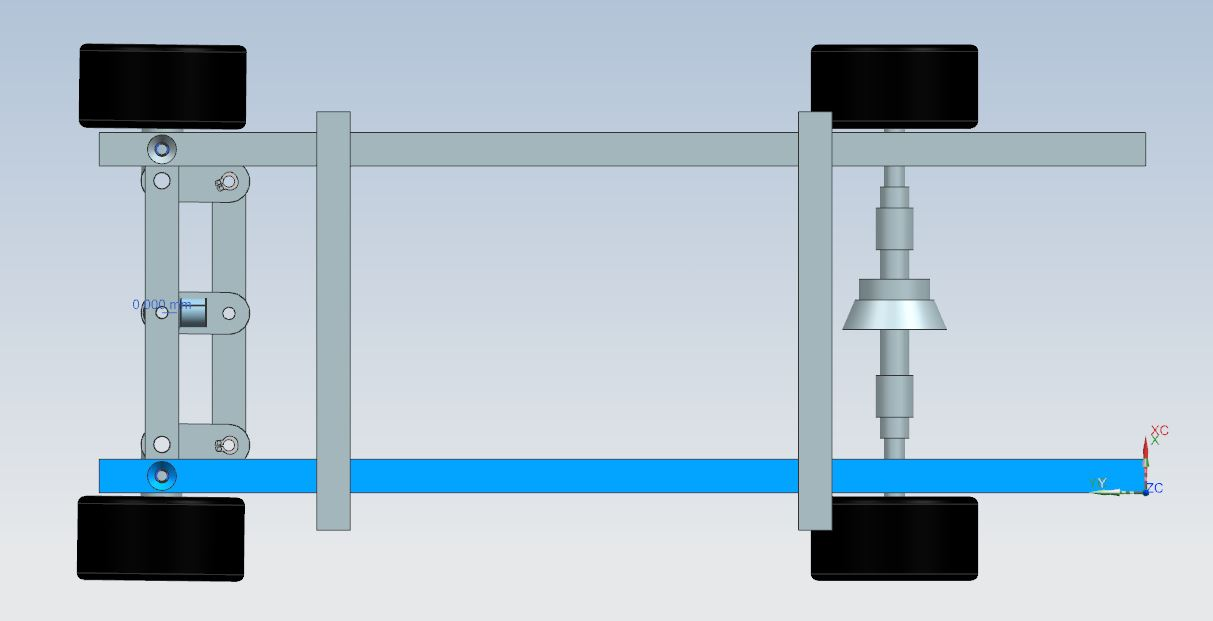
\includegraphics[width=\textwidth]{fig/4Rad-1.JPG}
		\caption{1. Situation: Ansicht von oben}
	\end{subfigure}
	\hfill
	\begin{subfigure}[b]{0.45\textwidth}
		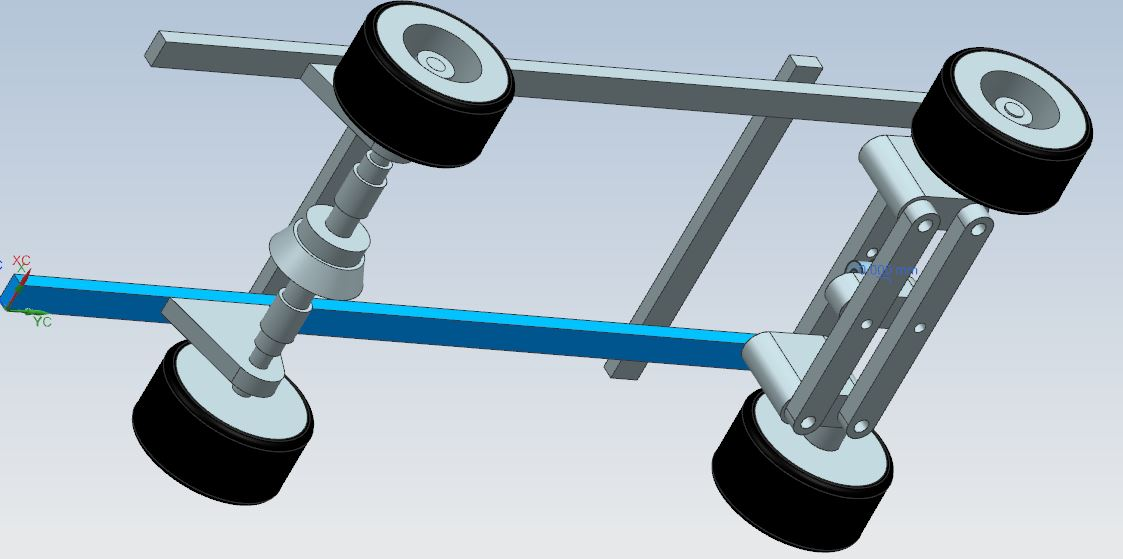
\includegraphics[width=\textwidth]{fig/4Rad-2.JPG}
		\caption{2. Situation: Ansicht von unten}
\end{subfigure}
	\caption{4-Rad mit Heckantrieb}\label{fig:animals}
\end{figure}

\begin{table}[h]
\begin{tabular}{p{0.5\textwidth} | p{0.5\textwidth}}


 \textbf{Vorteile} & \textbf{Nachteile} \\ \hline
	 
\begin{itemize}
\item Viel genutztes Prinzip im Modellbau
\item Viele Vorlagen im Internet
\item Klare Trennung zwischen Antrieb und Lenkung
\item Sehr Stabil
\end{itemize}

 
 &
 
\begin{itemize}
\item Für den Heckantrieb ist ein Differential notwendig
\item Es muss eine Lenkung eingebaut werden 
\item Regelung der Lenkung ist aufwendig
\end{itemize}

\end{tabular}
\end{table}

\begin{table}[h]
\begin{tabular}{p{0.5\textwidth}p{0.5\textwidth}}


 \textbf{Risiken} & \\ \hline
	 
\begin{itemize}
\item Ist das Fahrzeug zu lang, könnte man in der Kurve mit den Hinterrädern die Fahrbahn verlassen.
\end{itemize}
&
\begin{itemize}
\item Die Lenkung könnte zu unpräzise sein.
\end{itemize}

 
\end{tabular}
\end{table}

\pagebreak


%############## 3-Rad
\subsection{2-Rad mit Stützen}

\begin{figure} [hbp]
	\centering
	\begin{subfigure}[b]{0.4\textwidth}
		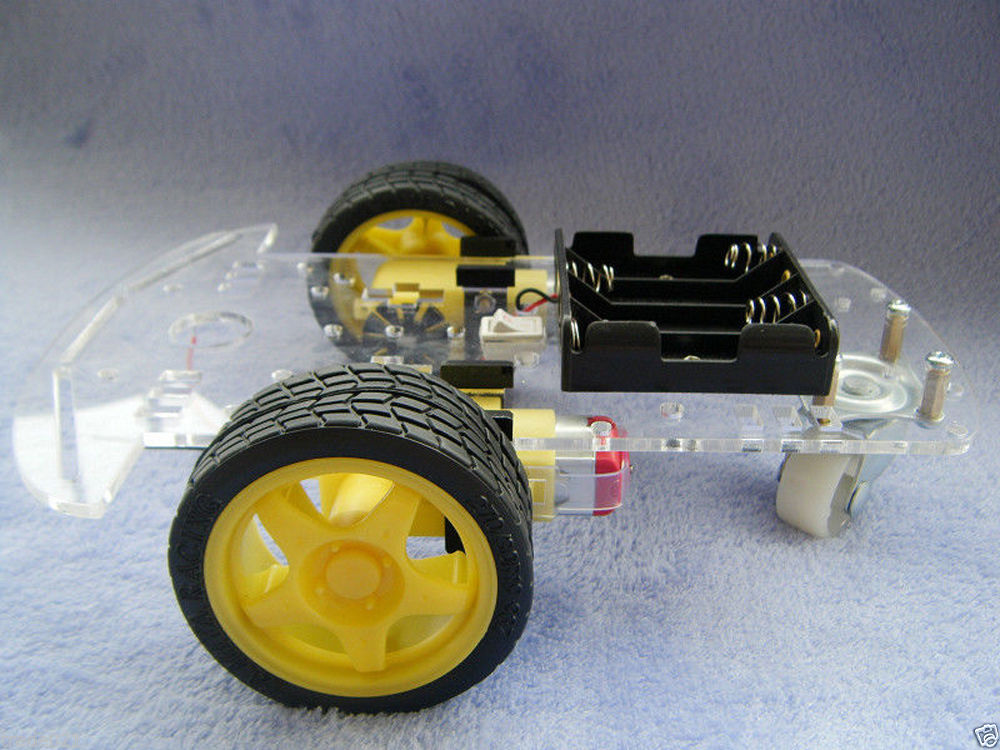
\includegraphics[width=\textwidth]{fig/3rad-1.jpg}
		\caption{1. Situation: Modell 
		(Quelle: www.sainsmart.com)}
	\end{subfigure}
	\hfill
	\begin{subfigure}[b]{0.36\textwidth}
		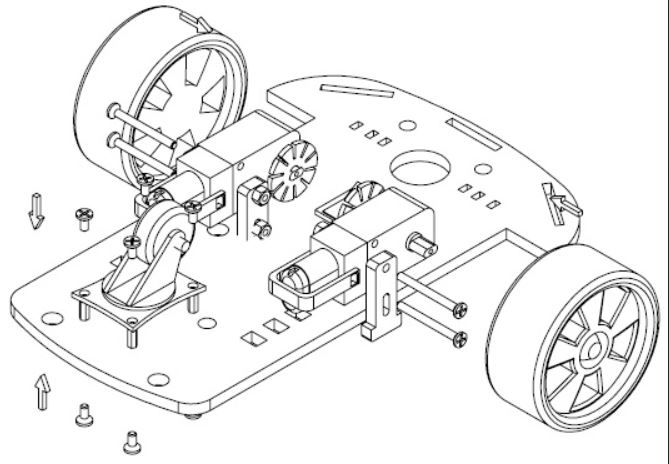
\includegraphics[width=\textwidth]{fig/3rad-3.JPG}
		\caption{2. Situation: Technische Zeichnung
		(Quelle: www.sainsmart.com)}
\end{subfigure}
	\caption{2-Rad Modell}\label{fig:animals}
\end{figure}

\begin{table}[h]
\begin{tabular}{p{0.5\textwidth} | p{0.5\textwidth}}


 \textbf{Vorteile} & \textbf{Nachteile} \\ \hline
	 
\begin{itemize}
\item Einfache Lenkung
\item Selber Motor für Antrieb und Lenkung
\item Sehr wendig
\item Konstruktiv einfach Realisierbar
\end{itemize}

 
 &
 
\begin{itemize}
\item Stabilität eher gering
\item Motoren müssen sehr genau sein
\item Grösse der Motoren für einen geeigneten Antrieb 
\end{itemize}

\end{tabular}
\end{table}

\begin{table}[h]
\begin{tabular}{p{0.5\textwidth}p{0.5\textwidth}}


 \textbf{Risiken} & \\ \hline
	 
\begin{itemize}
\item Bei einem 2-Rad Modell ist die Stabilität das grösste Problem. Beim Aufladen des Containers könnte das Fahrzeug kippen.
\end{itemize}
&
\begin{itemize}
\item Wenn die Antriebsräder in der Mitte montiert sind, braucht man vorne und hinten ein Stützrad oder eine Stützkugel. Diese könnten grössere Reibungskräfte verursachen.
\end{itemize}

 
\end{tabular}
\end{table}

\pagebreak
% !TEX root = ../Dokumentation.tex
\subsection{Lenkung}

\textbf{Funktionsbeschrieb}
\\[0.2cm]
Die Lenkung ist eine Achsschenkellenkung. Sie wird heute in fast allen PKWs, LKWs, Omnibussen und sonstige Nutzfahrzeugen eingesetzt. Bei dieser Art der Lenkung befinden sich die Räder auf einzeln lenkbaren Achsschenkeln, die jeweils mit einem Spurstangenhebel versehen sind. Die Spurstangenhebel sind ungefähr senkrecht zur Vorderachse bzw. ungefähr parallel zur Längsachse des Fahrzeugs ausgerichtet und mittels einer Spurstange miteinander verbunden. Dadurch werden beide Räder gleichzeitig gelenkt.\\[0.2cm]
\textbf{Komponentenbeschrieb}
\\[0.2cm]
Mit einem Servomotor wird über eine Kegelradverbindung der Lenkschubhebel angetrieben. Dieser treibt wiederum die Spurstange an, welche die Bewegung Über die Spurstangenhebel an die Räder weitergibt.
\begin{figure}[H]%Position festigen
\centering
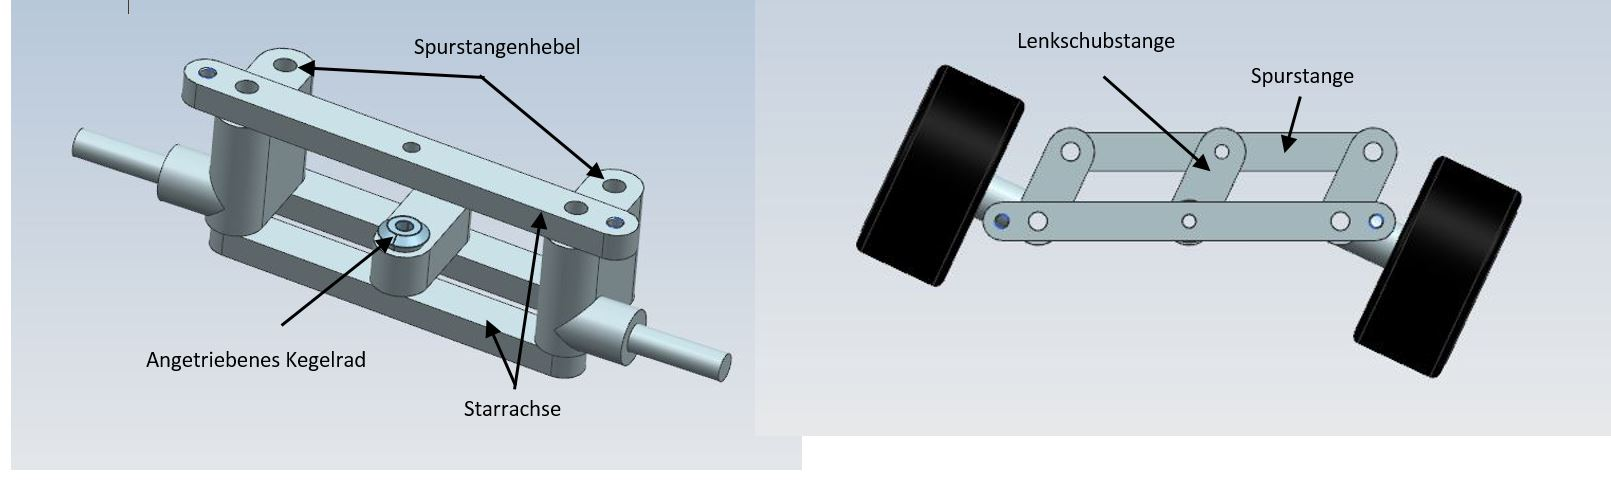
\includegraphics[width=1\textwidth]{03_Loesungskonzept/pictures/Achsschenkellenkung.JPG}
\caption{Konzept der Achsschenkellenkung}
\label{fig:activityRoute}
\end{figure}
\textbf{Begründung}\\[0.2cm]
Für die Bildverarbeitung ist das Lenken und konstante ausgleichen der Fahrbahn und Fahrtgeschwindigkeit mit zwei Motoren, welche jeweils ein Rad antreiben Nachteil. Darum ist das Lösungskonzept mit einer Achsschenkellenkung ausgestattet. Von der Konstruktiven seit ist die Achsschenkellenkung im Vergleich zwar aufwändiger aber für die Aufgabenstellung besser geeignet. Da dass Ziel ist einen möglichst konstanten Abstand zum Trottoir der Fahrbahn zu halten, ist die Regelung einer Achsschenkellenkung einfacher. Weitere Gründe, welche für die Achsschenkellenkung sprechen wurden schon im Kapitel \glqq{Chassis}\grqq  erläutert.
Die Begründung für die Wahl des Servomotors ist, dass die Lenkung keine 360° Bewegungen durchführen muss. Zudem ist die Drehzahl des Servos leicht zu steuern, ohne das zusätzlich eine Regelung eingebaut werden muss. 
\textbf{Berechnungen}\\[0.2cm]
Berechnung Drehmoment Servo Lenkung
Gewichtskraft auf jedes Rad Fg = m*g/4
Abstand l = 30mm
M = 2*Fg*l = 0.37Nm
Sicherheitsfaktor = 1.5 (da Beschleunigung- und Bremskräfte vernachlässigt werden)
M = 0.37*1.5 = 0.555Nm = 55.5Ncm\flushleft
% !TEX root = ../Dokumentation.tex
\subsection{Antrieb}

\textbf{Funktionsbeschrieb}\\[0.2cm]
Als Antrieb wird ein DC-Getriebemotor verwendet, der an der Unterseite montiert wird und für die Vor- sowie Rückwärtsbewegungen des Fahrzeugs zuständig ist.
Die aktuelle Drehzahl des Motors wird von einem Encoder erfasst. Dieser wiederum sendet die gemessenen Daten an den Microcontroller der schlussendlich die Anzahl Umdrehungen reguliert.\\[0.2cm]
\textbf{Komponentenbeschrieb}
\begin{figure}[H]
\centering
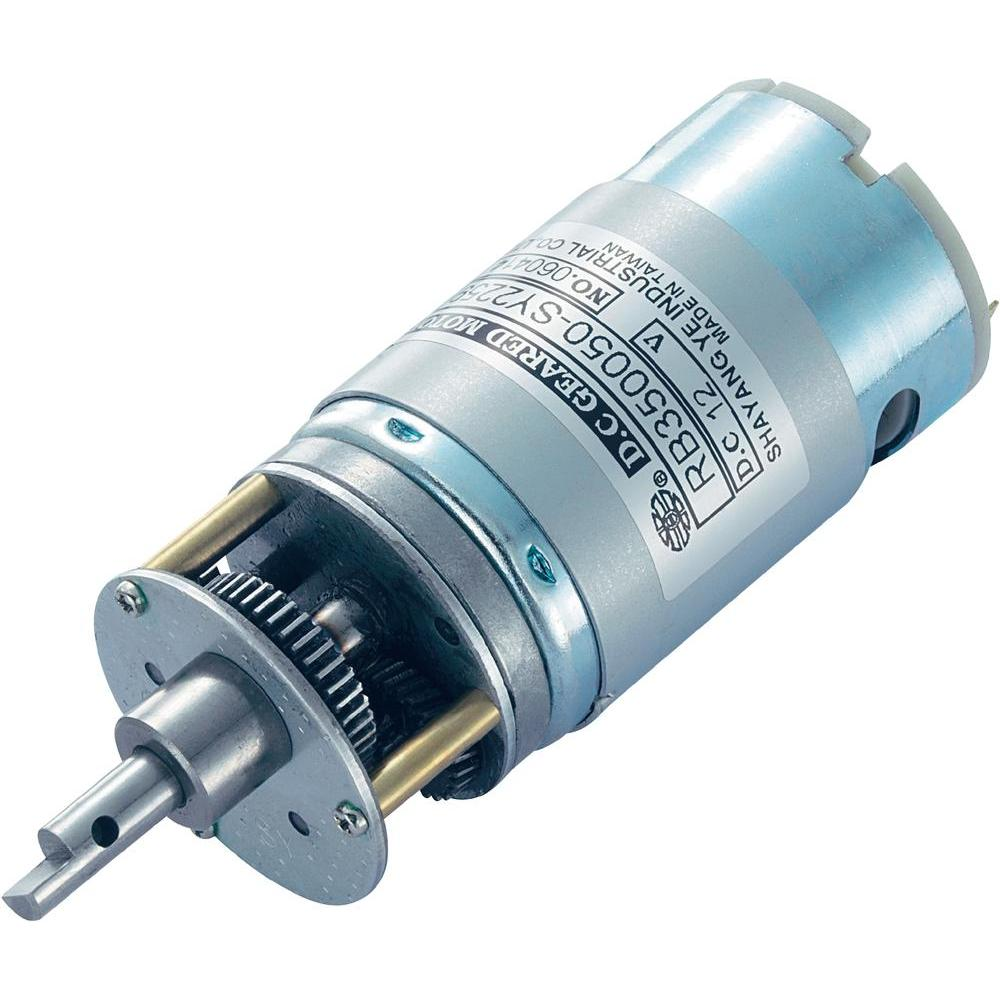
\includegraphics[width=0.5\textwidth]{03_Loesungskonzept/pictures/antrieb.jpg}
\caption{Antrieb  (Quelle:http://www.conrad.ch)}	
\end{figure}\flushleft
Als voraussichtlicher Favorit wurde ein Hochleistungsgetriebemotor von Modelcraft ausgewählt. Die technischen Daten sind folgende:
\begin{itemize}
\item Leerlaufstrom: 0.32 A
\item Last-Drehzahl: 317 U/min
\item Leerlauf-Drehzahl: 333 U/min
\item Betriebsspannung: 12 V DC
\item Spitzendrehmoment: 2.23 Nm
\item Max. Laststrom: 0.7 A
\end{itemize}
\textbf{Begründung}\\[0.2cm]
Der ausgewählte Motor punktet vor allem aufgrund seiner kleinen und kompakten Bauform. Da der Montageort für den Antrieb am Fahrzeug nicht verändert werden kann, ohne umständliche Wellen zu installieren, ist die Baugrösse relativ beschränkt.
Ein weiterer Punkt ist, dass er sich als Gleichstrommotor leicht ansteuern lässt und damit die Handhabung vereinfacht.
Zudem zeichnet er sich mit einer hohen Drehzahl und grossem Drehmoment aus und ist dennoch verhältnismässig günstig in der Anschaffung.

% !TEX root = ../Dokumentation.tex
\subsection{Beladen und Greifer}

\textbf{Funktionsbeschrieb}
\begin{figure}[H]
\centering
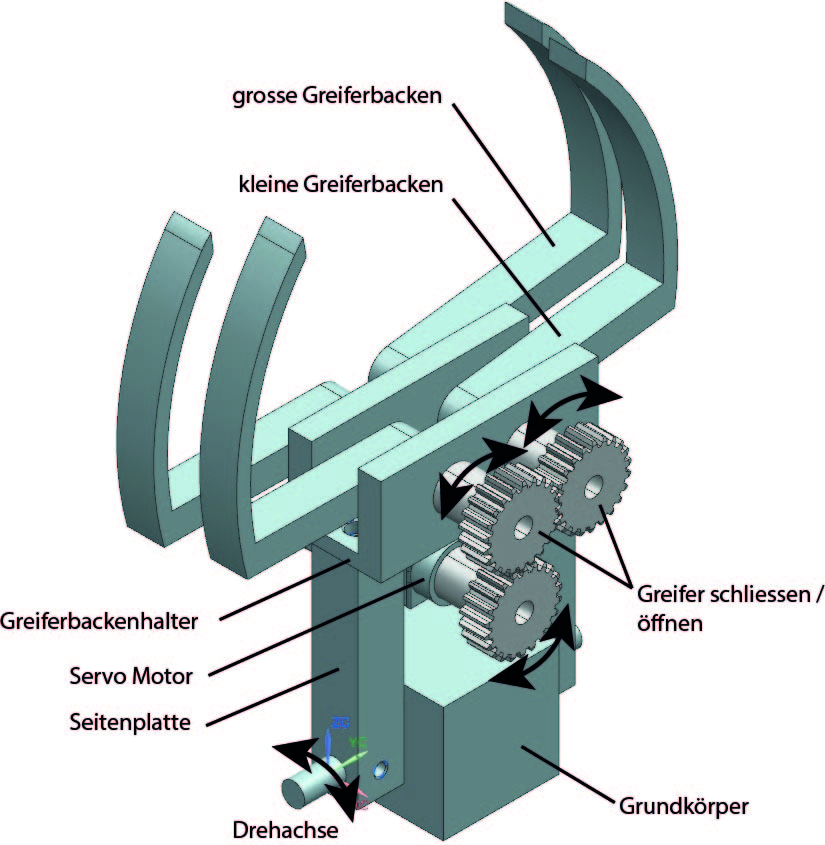
\includegraphics[width=0.5\textwidth]{03_Loesungskonzept/pictures/greifer3.jpg}
\caption{Greifer}
\end{figure}\flushleft

Der Greifer ist auf der Grundplatte des Fahrzeuges montiert. Im Grundkörper wird die Welle für die Drehung des Greifers montiert. Die Welle wird von einem Servo Motor angetrieben. Um gute Laufeigenschaften zu erreichen werden Lagerbüchsen eingebaut. Auf der Drehachse sind die beiden Seitenplatten des Greifers montiert. Auf den Seitenplatten wird der Greifbackenhalter verschraubt.  Der Servo Motor für die Funktion Greifer schliessen/ öffnen wird am Greifbackenhalter befestigt. Auf dem Servo wird ein Zahnrad montiert, das über die gleichen Zahnräder die Greiferbacken öffnet bzw. schliesst. Die Greiferbacken sind so konzipiert, dass die 2 längeren und 2 kürzeren an verschiedenen Flächen greifen. Damit wird erreicht, dass der Container stabil bleibt während des ganzen Einladeprozesses. 

\begin{figure}[H]
\centering
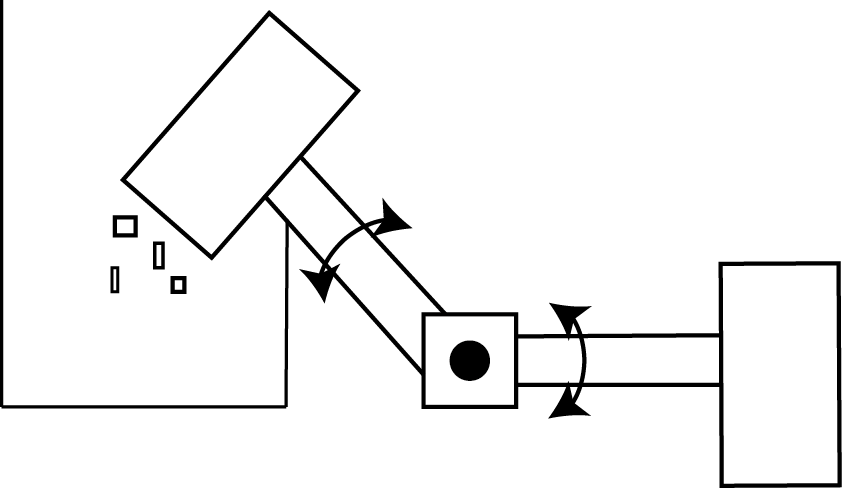
\includegraphics[width=0.5\textwidth]{03_Loesungskonzept/pictures/Beladen_1.png}
\caption{Einladeprozess}
\end{figure}\flushleft
Der Greifer ist während des Fahren in oberer Position gelagert, damit die Abmasse der Aufgabenstellung eingehalten werden können. Der Greifer wird erst auf horizontale Richtung bewegt, nachdem der Wagen still steht und richtig positioniert ist.
Die rechte Fahrzeugkante wird auf 25mm +/- 5mm zum Trottoirrand positioniert. In Fahrtrichtung beträgt die maximale zulässige Positionierungsgenauigkeit +/- 10mm.

\begin{figure}[H]
\centering
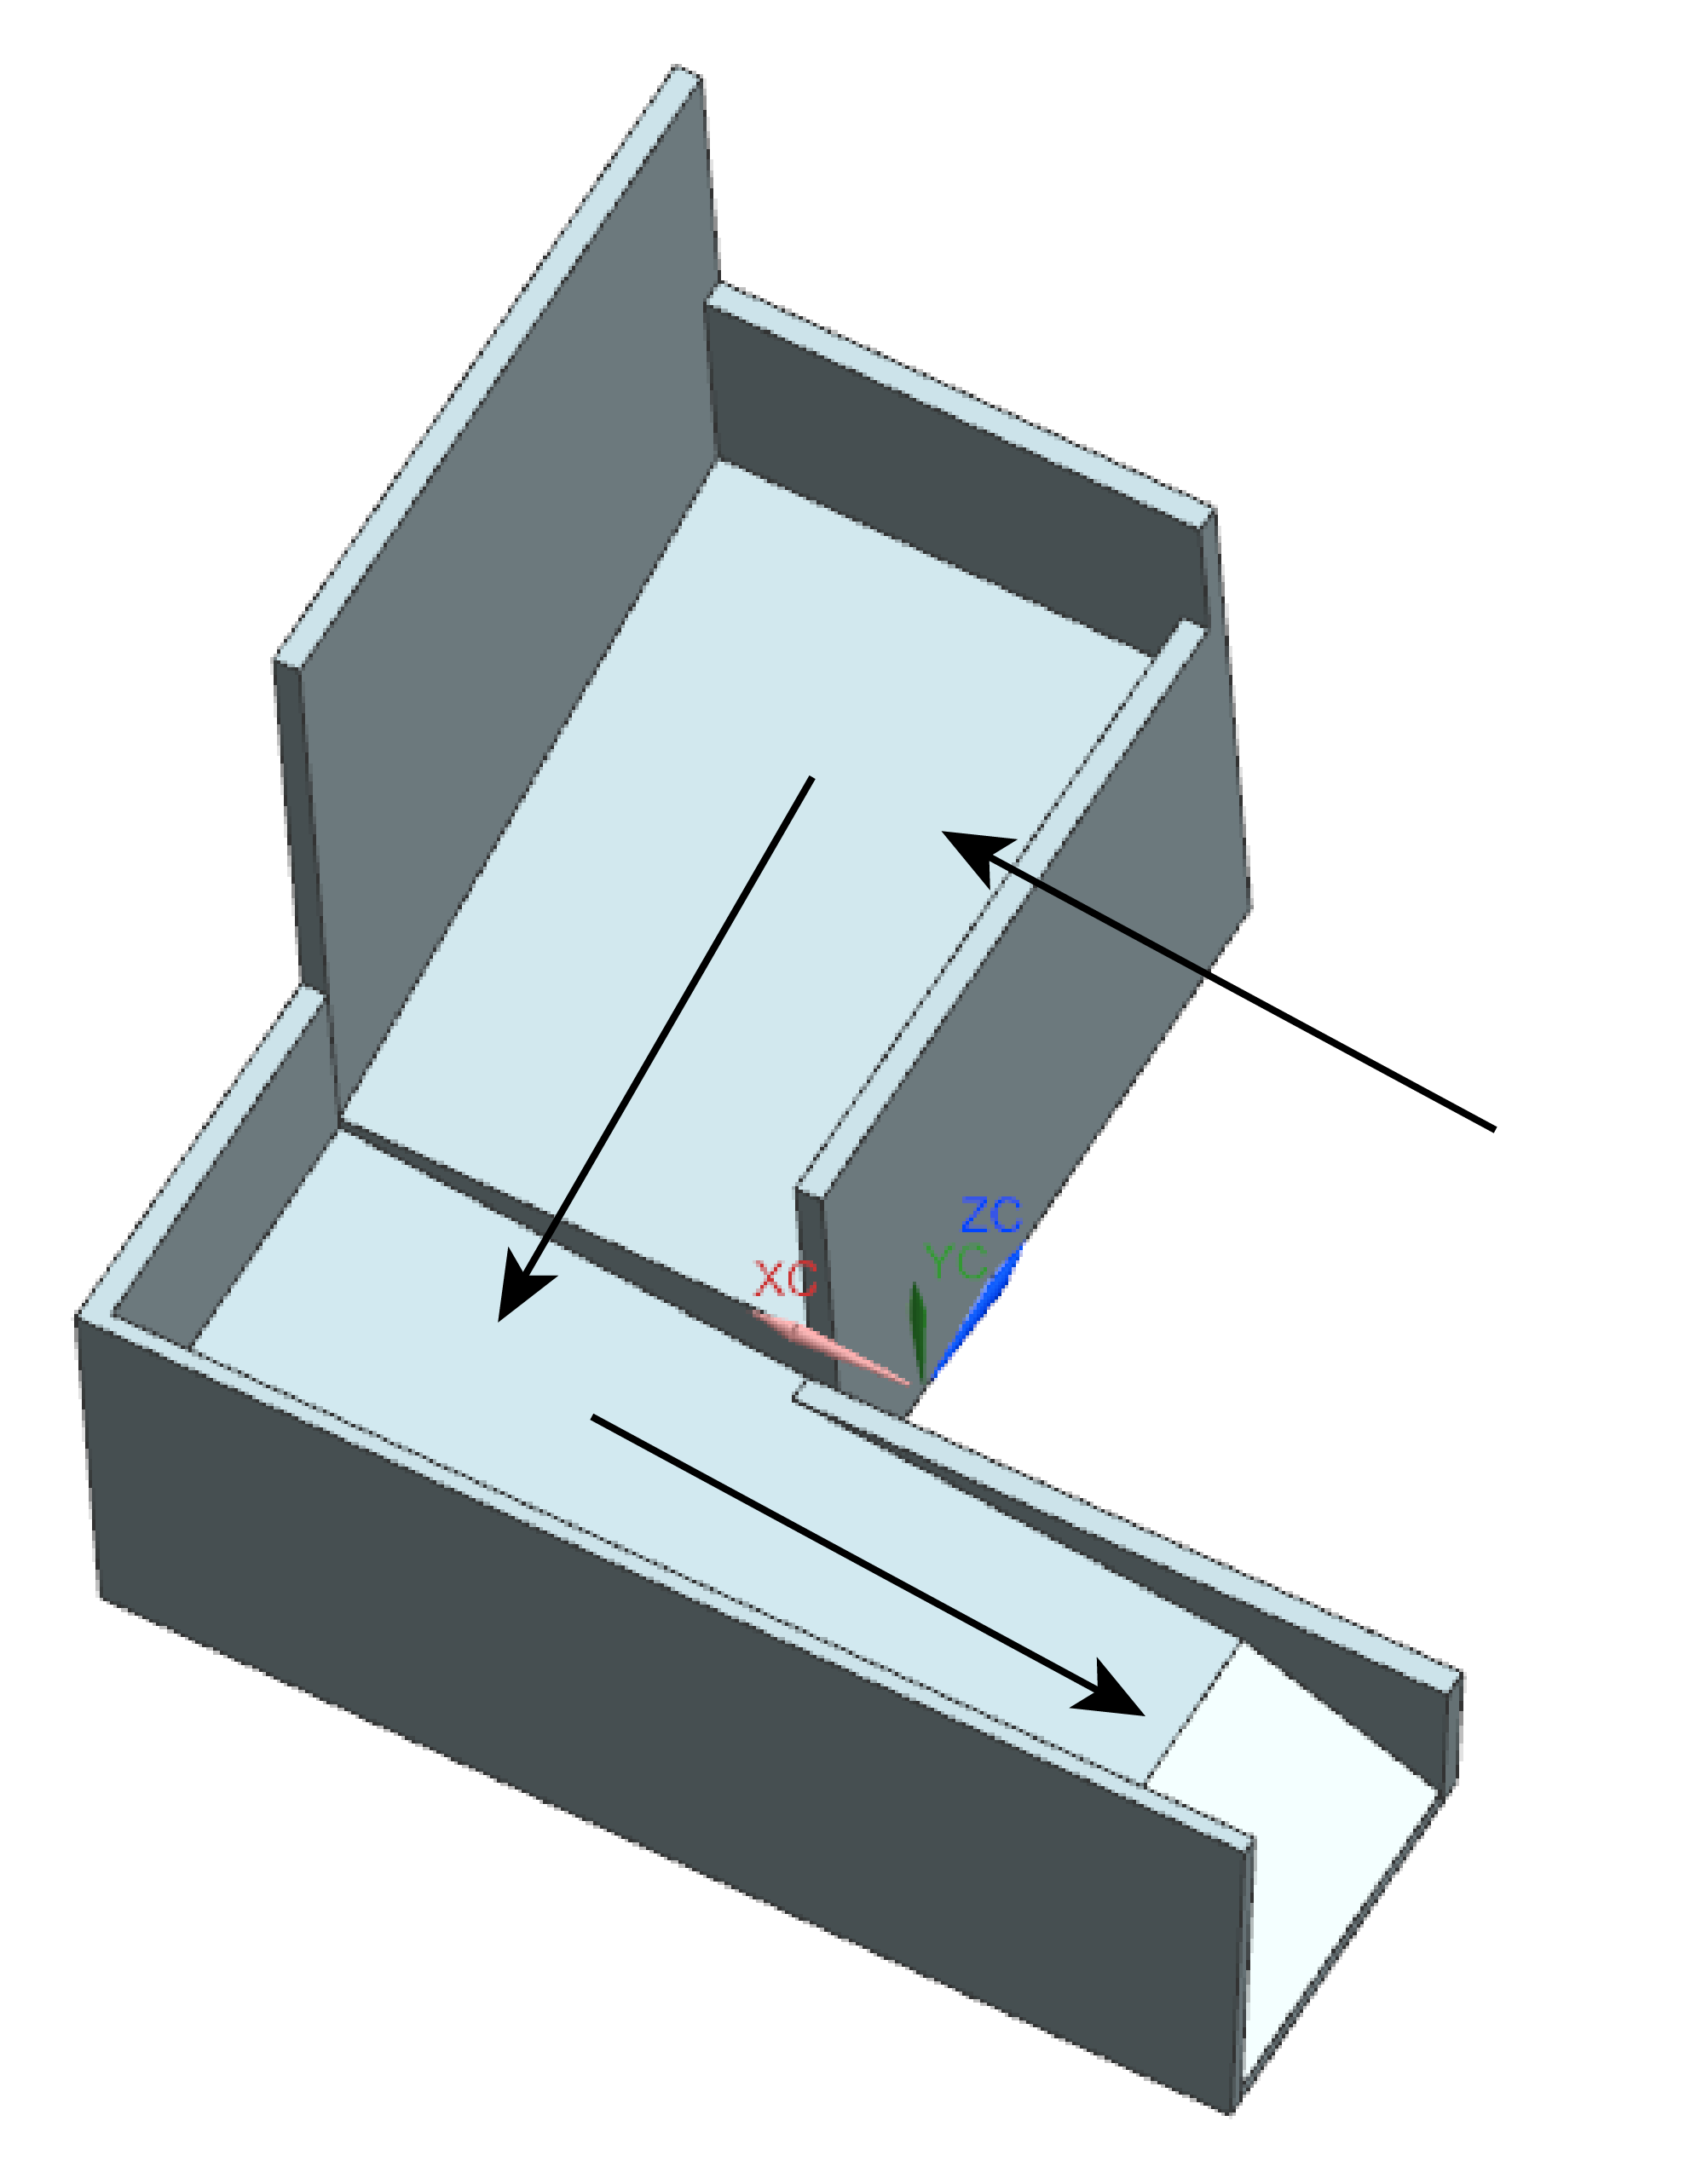
\includegraphics[width=0.5\textwidth]{03_Loesungskonzept/pictures/behaelter.png}
\caption{Schüttgutfluss in den beiden Behältern}
\end{figure}\flushleft
Der Container wird in den ersten Behälter entleert. Durch den schrägen Boden rutscht das Schüttgut in den zweiten Behälter. Am Ende des zweiten Behälters wird ein Klappe montiert, damit die Schrauben und Mutter nicht herausfallen. Die Klappe wird durch einen Servo Motor gehalten und erst am Schluss beim Entladebehälter geöffnet.\\[0.2cm]

\textbf{Komponentenbeschrieb}\\[0.2cm]
\begin{itemize}
\item Zahnräder aus Kunststoff, Durchmesser = 15 (Einkaufteil)
\item Greiferbacken aus Kunststoff (Druckteil)
\item Grundkörper, Seitenplatte, Greifbackenhalter und Wellen werden aus Aluminium gefertigt.
\item Behälter aus Acrylglas 3mm Dicke (Laserzuschnitt)
\item Technische Daten des Motors Greifer:
\begin{itemize}
\item Stellzeit bei 4.8 Volt: 0.1 sec (50°) 
\item Stellzeit bei 6 Volt: 0.08 sec (50°) 
\item Betriebsspannung: 4.6/6 V
\item Stell-Moment bei 4.8 Volt: 18 Ncm
\item Stell-Moment bei 6 Volt: 20 Ncm 
\end{itemize}
\end{itemize}
\textbf{Berechnungen}\\[0.2cm]
Servo Motor für Greifer schliessen /
Berechnung des benötigten Drehmoments: 
\begin{itemize}
\item Haftreibung auf 0.7 geschätzt
\item Masse Container $m = 0.075kg$
\item Gewichtskraft = $m\cdot g = 0.74 N$
\item Kraft $F = \frac{0.5\cdot 0.74}{0.7} = 0.53 N$
\item Abstand $l = 80mm$ (Drehpunkt zu Greiffläche)
\item $M = F\cdot l = 0.04 Nm = 4 Ncm$
\item Sicherheitsfaktor = 2
\item M = $4\cdot 2 = 8 Ncm$
\end{itemize}
Servo Motor für Greifarm drehen:
\begin{itemize}
\item Gewichtskraft Container $Fc = 0.075kg\cdot 9.81 = 0.74 N$
\item Gewichtskraft Greifarm: $Fgr = 0.3kg\cdot 9.81 = 2.94 N$
\item Benötigtes Moment:
$M = Fgr\cdot 0.05m+Fc\cdot 0.1m = 0.147Nm+0.07Nm = 0.217Nm = 21.7Ncm$
\item Sicherheitsfaktor = 2 wegen Abschätzug des Greifergewichts und vernachlässigter Trägheitskräfte
\item $M = 2 \cdot 21.7 = 43.4 Ncm$
\end{itemize}
% !TEX root = ../Dokumentation.tex
\subsection{Entladen}

\textbf{Funktionsbeschrieb}\\[0.2cm]
\begin{figure}[H]
\centering
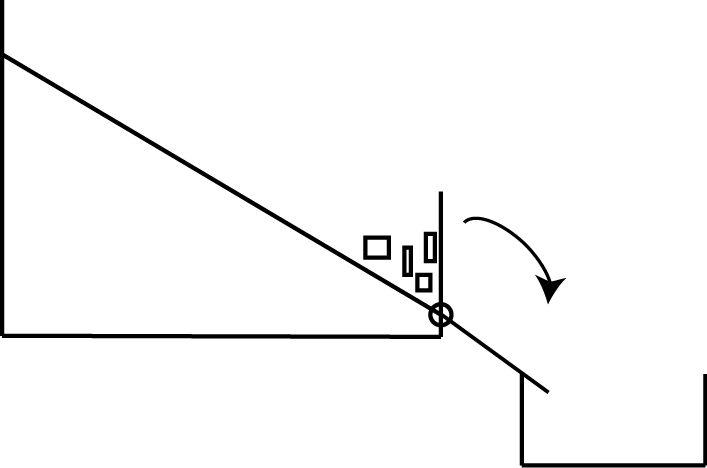
\includegraphics[width=0.5\textwidth]{03_Loesungskonzept/pictures/Entladen_Schraegbehaelter.png}
\caption{Entladen}
\end{figure}

\ Beim Entladevorgang fährt das Fahrzeug bis auf 20mm +/- 5mm an den Rand des Entsorgungsbecken. Anschliessend wird die Klappe gelöst und diese fällt auf den Rand des Entsorgungsbecken. Über die Klappe rutscht das Schüttgut in das Entsorgungsbecken. Nach erfolgter Abladung fährt das Fahrzeug kurz nach links, damit das ganze Fahrzeug im Zielbereich steht. Dabei hängt die Klappe nach unten.

\textbf{Komponentenbeschrieb}

\ Die Klappe besteht aus einem handelsüblichen Scharnier auf dem eine Platte aus Acrylglas befestigt ist.
Die Klappe wird durch einen Servomotor gehalten.\\
Technische Daten des Servomotors:
\begin{itemize}
\item Stellzeit bei 4.8 Volt: 0.1 sec (50°) 
\item Stellzeit bei 6 Volt: 0.08 sec (50°) 
\item Betriebsspannung: 4.6/6 V
\item Stell-Moment bei 4.8 Volt: 18 Ncm
 \item Stell-Moment bei 6 Volt: 20 Ncm 
\end{itemize}

\textbf{Berechnungen}
\ Die Berechnungen zum Servo Motor für die Klappe sind schon im Kapitel Beladen zu finden.
% !TEX root = ../Dokumentation.tex
\subsection{Halterungen}
\begin{figure}[H]
\centering
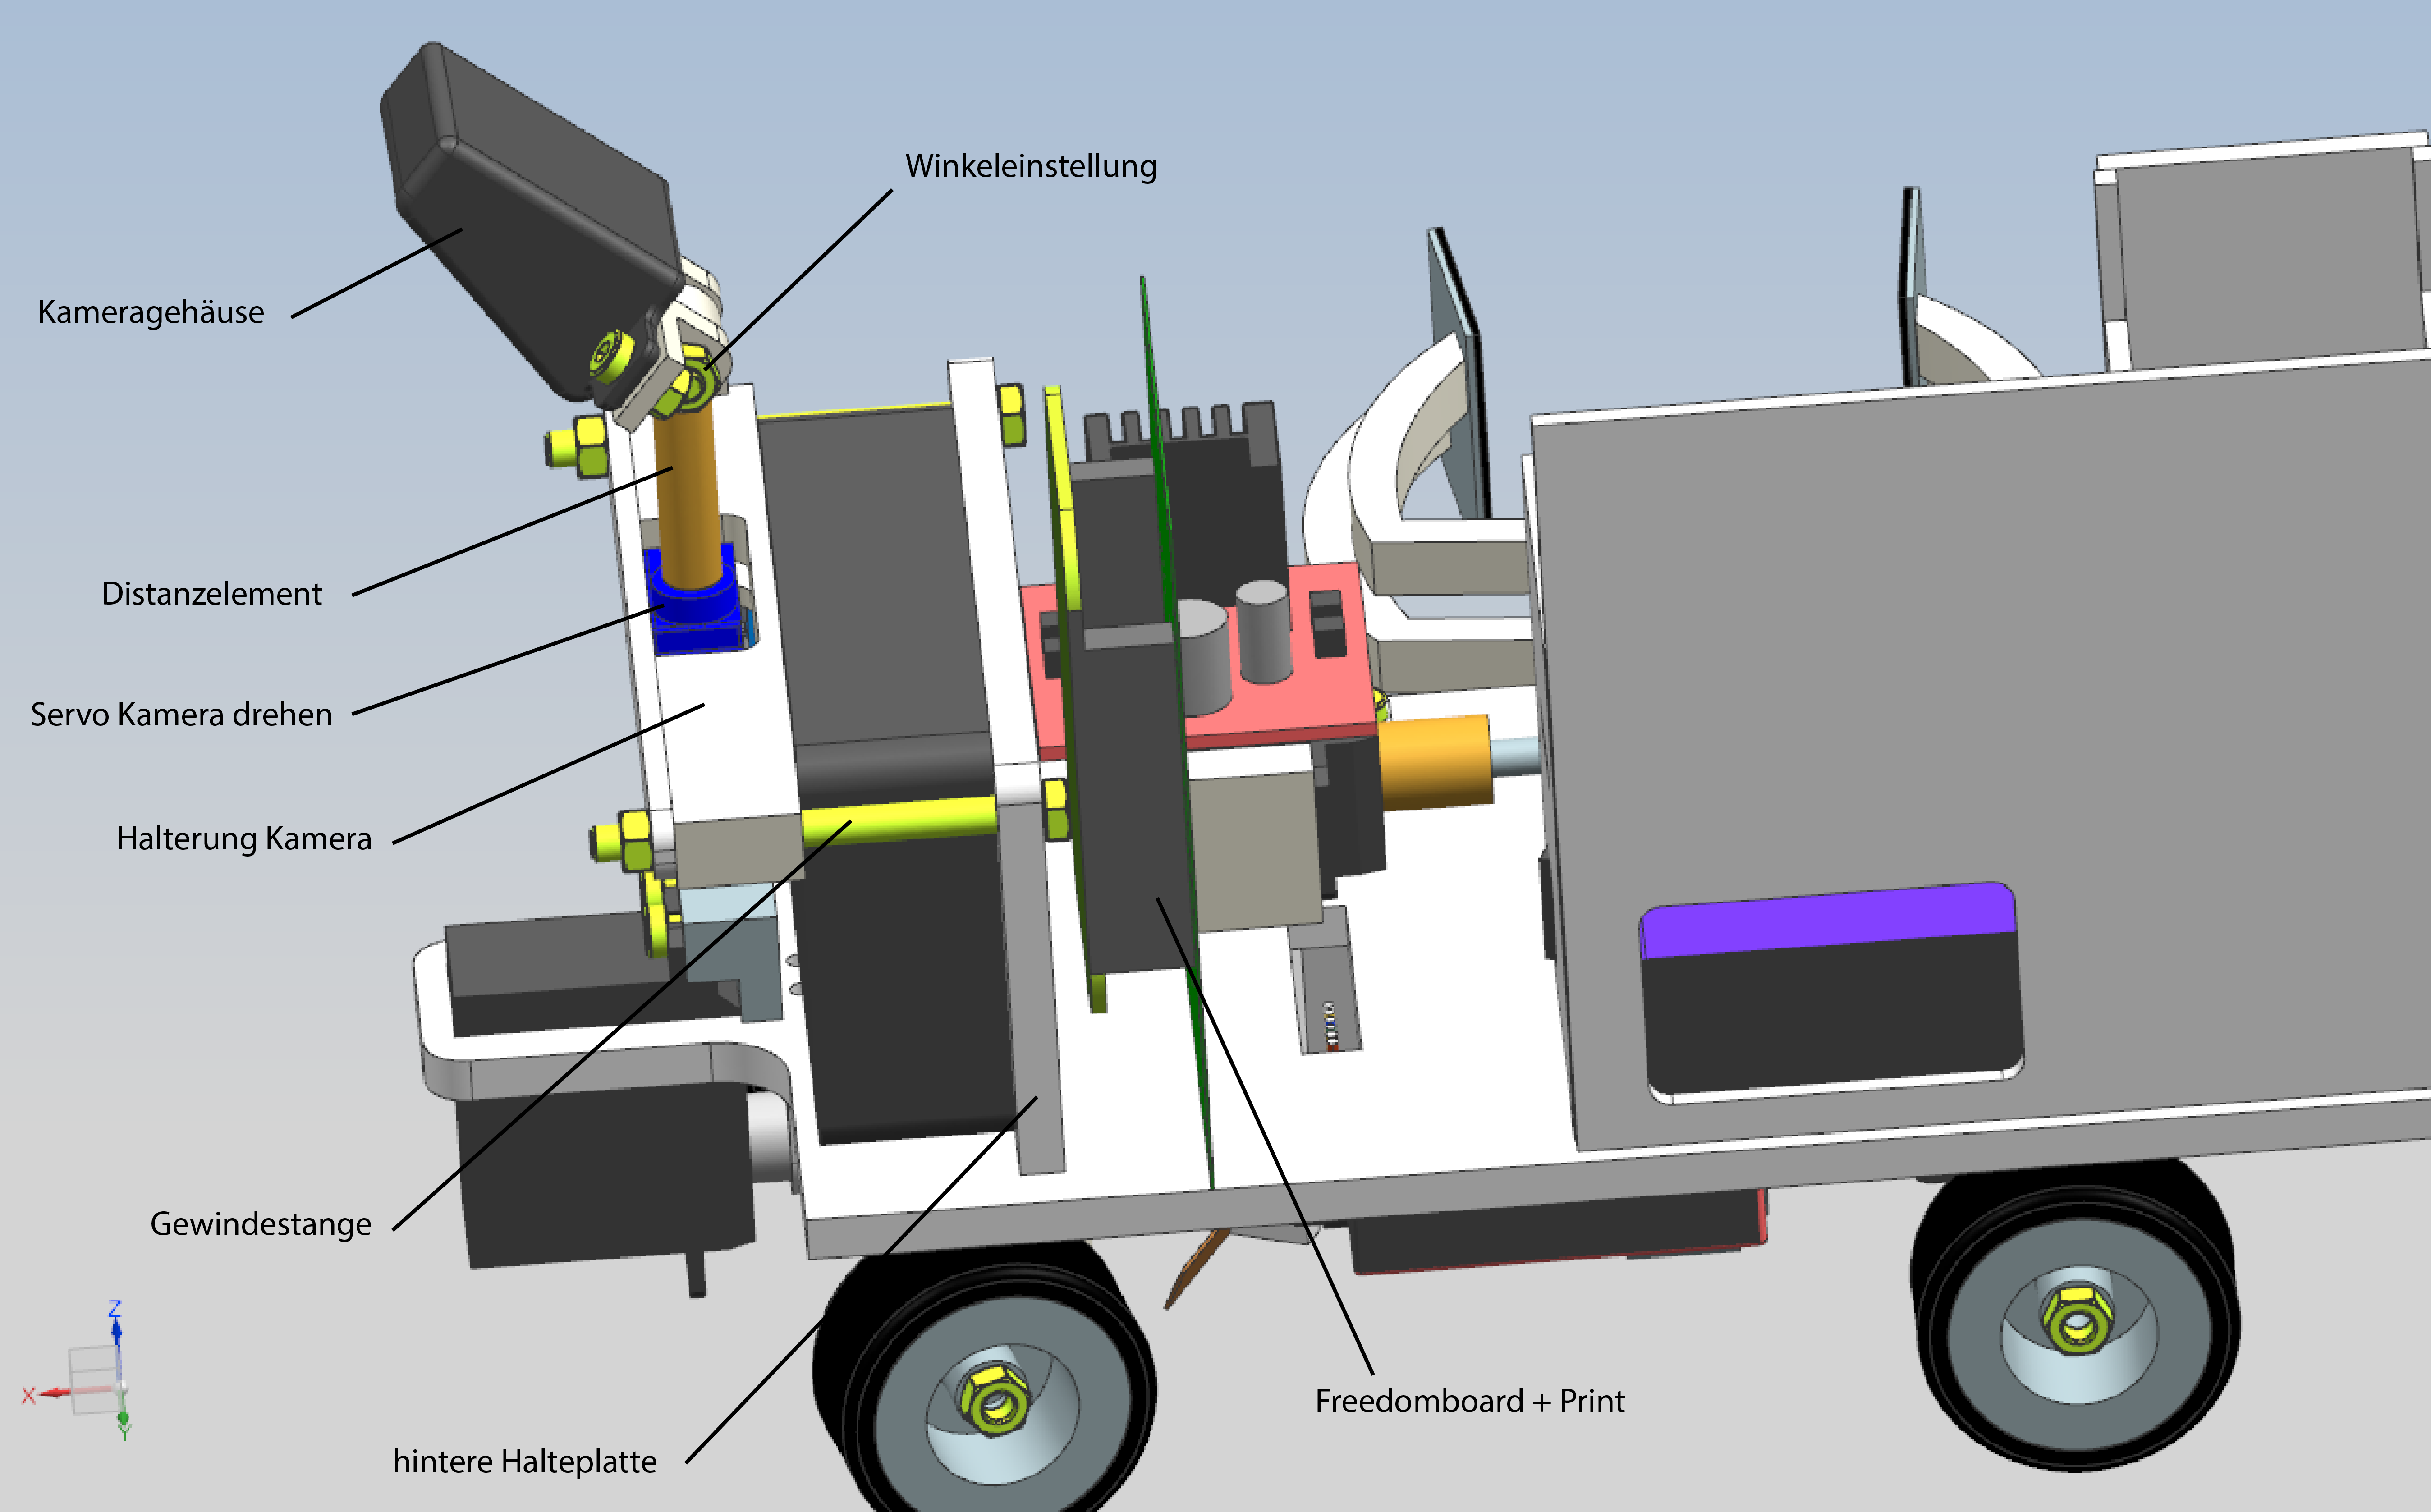
\includegraphics[width=1\textwidth]{03_Loesungskonzept/pictures/halterungen2.png}
\caption{Halterungen für Kamera, Rasperry Pi, Freedom Board und Print}
\end{figure}
\textbf{Halterung Kamera}\\[0.2cm]
Die Kamera ist auf einer festen Höhen montiert. Der Winkel zur Fahrbahn ist einstellbar. Nach Tests wurde der Winkel definitiv bestimmt und eingestellt.\\[0.2cm]
Die Kamera ist über ein Distanzelement auf dem Servo Motor montiert. Damit kann die Kamera in der Kurve gedreht werden. Der Servo Motor wird auf die Halterung (3D Druckteil) geschraubt.\\[0.2cm]
\textbf{Befestigung Rasperry Pi}\\[0.2cm]
Das Rasperry wird bei der Montage an die hintere Halteplatte gedrückt, die aus Acrylglas gefertigt ist und auf der Grundplatte angeschraubt ist. Auf der vorderen Seite wird ein 3D Druckteil und ein Acrylglasteil angebracht. Die beiden Seiten werden mit durchgehender Gewindestangen verschraubt. Dabei muss darauf geachtet werden, dass nicht zu stark angezogen wird um keine Teile zu beschädigen.\\[0.2cm]
\textbf{Befestigung Freedom Board und Print}\\[0.2cm]
Der Print und das Freedom Board wurden mit Klettverschluss auf der hinteren Halterungen des Rasperry PIs befestigt.\\[0.2cm]
\begin{figure}[H]
\centering
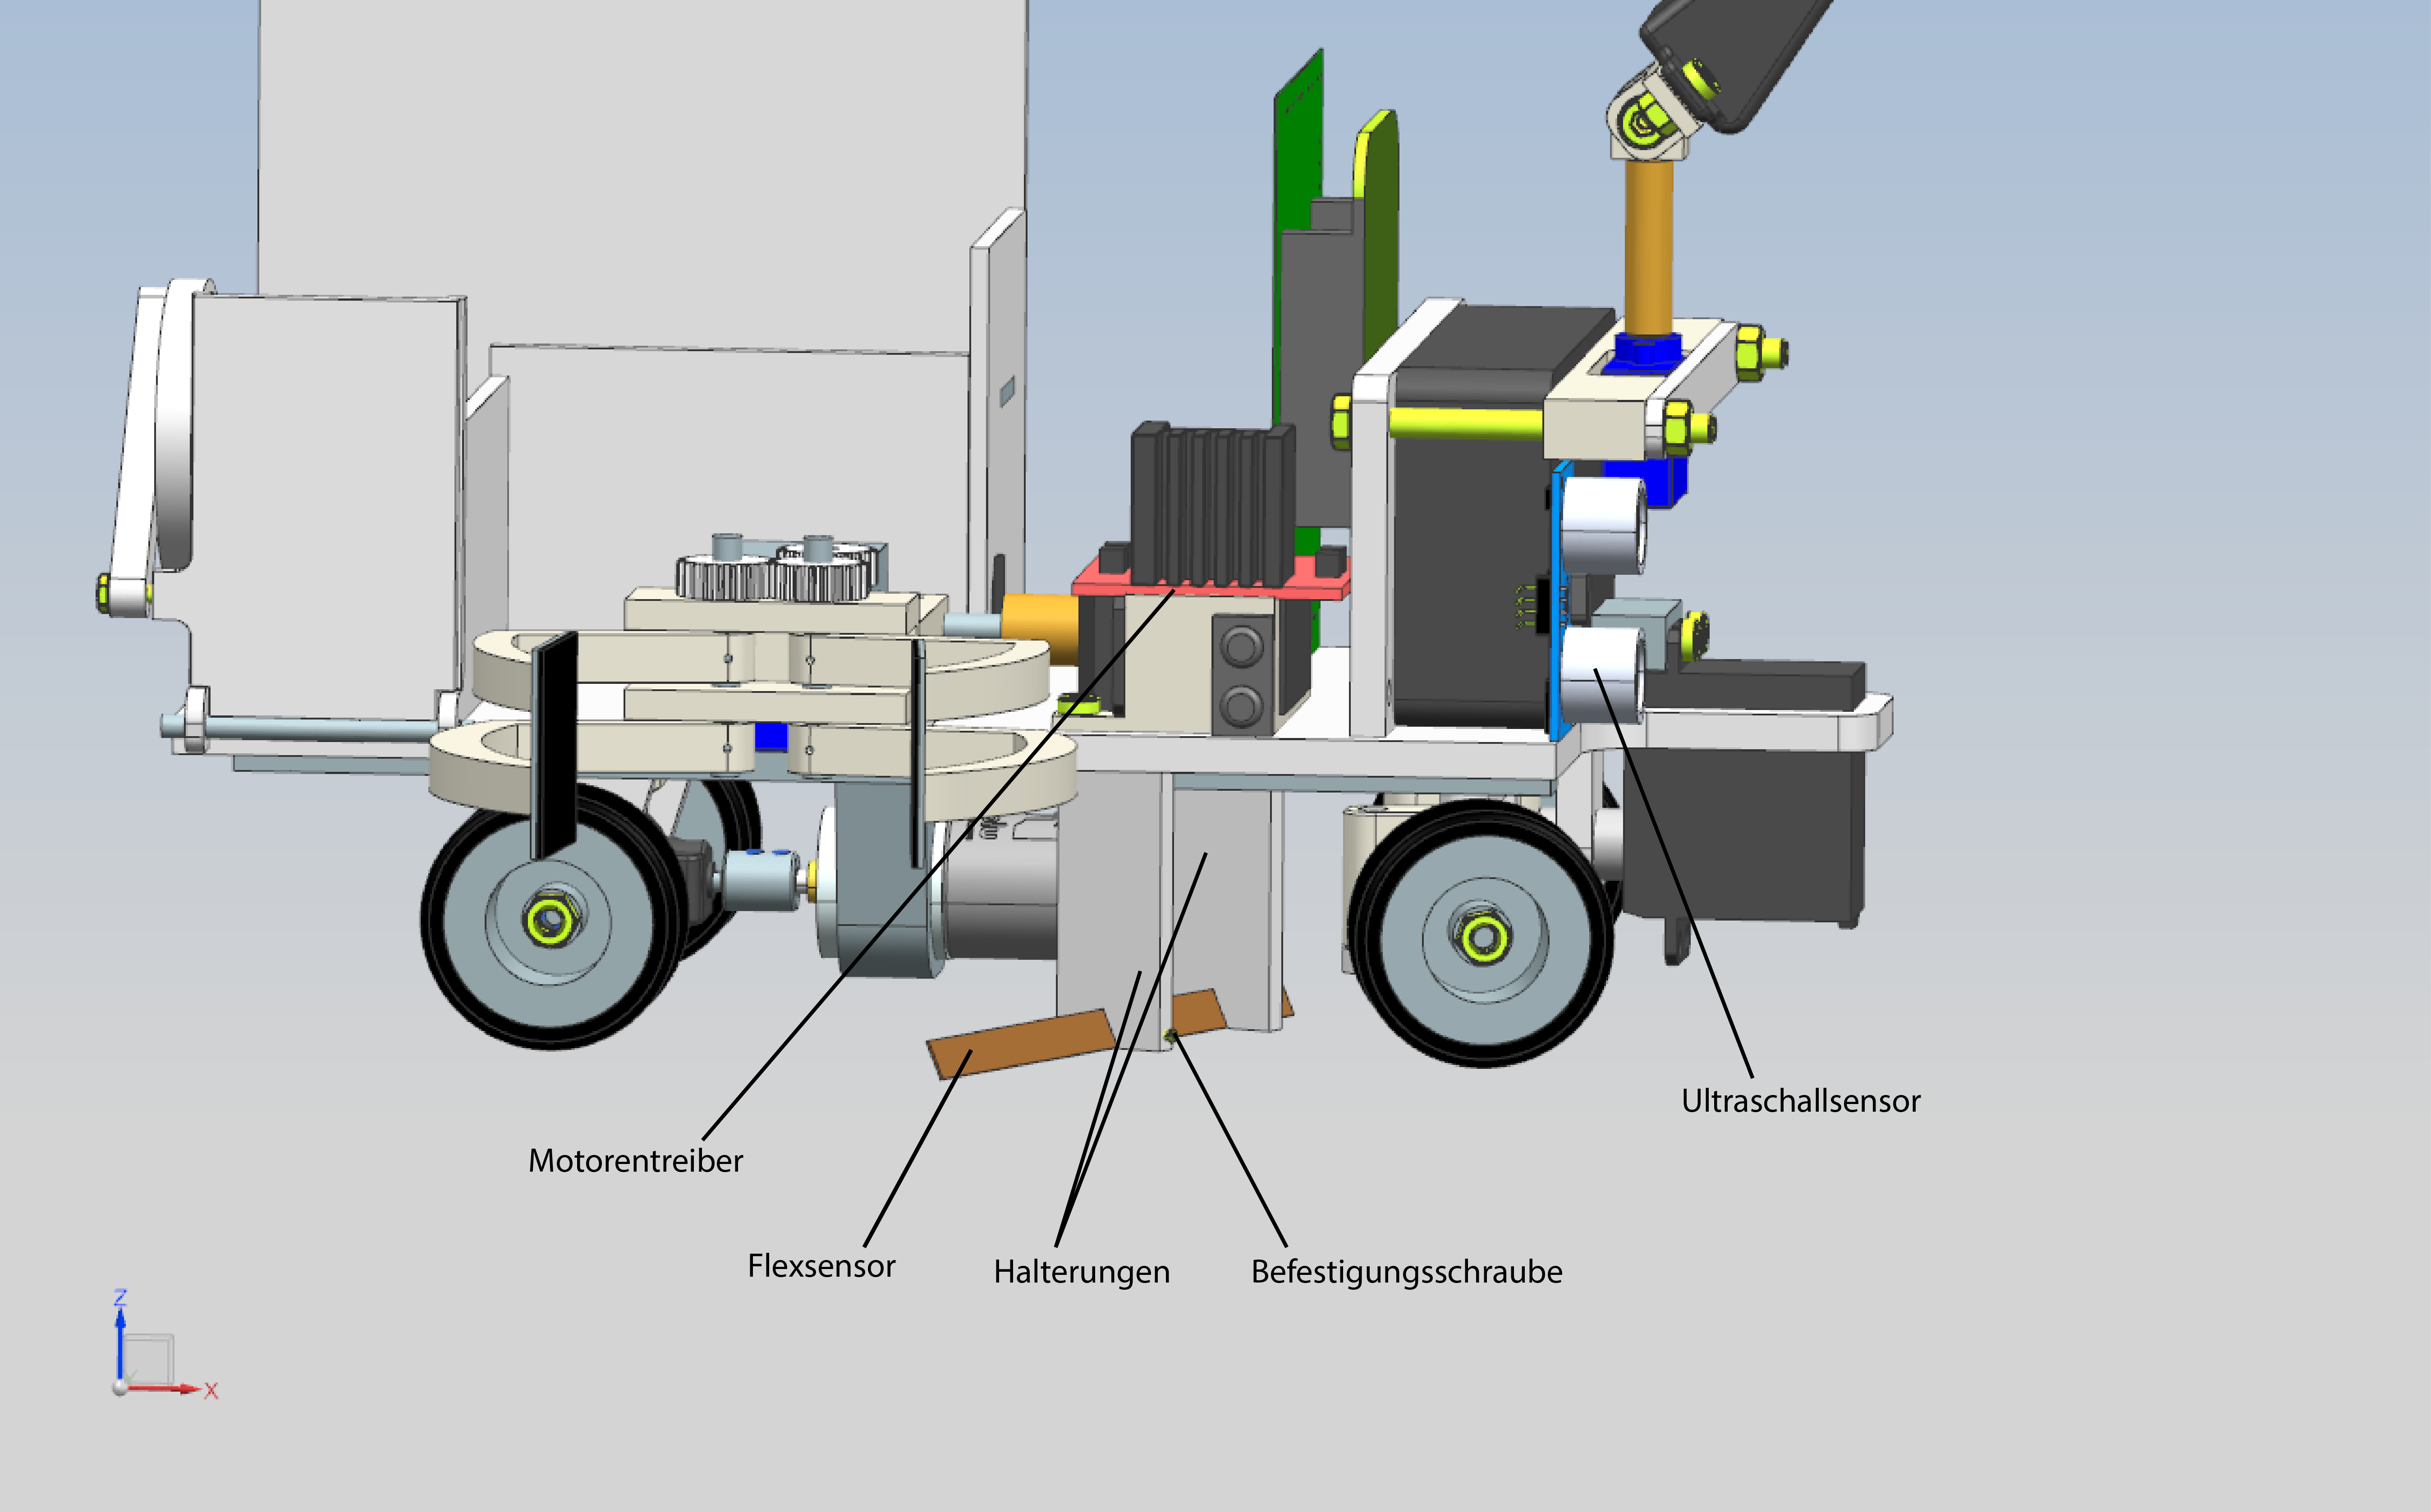
\includegraphics[width=1\textwidth]{03_Loesungskonzept/pictures/halterungen1.png}
\caption{Halterungen für Motorentreiber, Infrarotsensor und Flexsensor}
\end{figure}
\textbf{Befestigung Motorentreiber, Ultraschallsensor}\\[0.2cm]
Der Motorentreiber wurde mit Klettverschluss auf der Halterung für den Greifer drehen befestigt.\\[0.2cm]
Der Ultraschallsensor wird vorne rechts angeklettet.\\[0.2cm]
\textbf{Befestigung Flexsensor}\\[0.2cm]
Der Flexsensor wird unterhalb der Grundplatte montiert. Die zwei Halterungen wurden aus Acrylglas gelasert und unter die Grundplatte geklebt. Dabei sind die Halterungen leicht schräg. Der Flexsensor wird in die beiden Schlitze der Halterungen eingeführt. Um immer die gleiche Länge zu haben, kann der Flexsensor mit einer Schraube befestigt werden.\\[0.2cm]
\textbf{Befestigung Infrarot Sensor}\\[0.2cm]
Der Infrarot Sensor wurde auf der rechten Seite des Fahrzeugs auf die Halterung des Motors (Greifer drehen) angeklettet.
% !TEX root = ../Dokumentation.tex
\subsection{Energieversorgung}
%
\textbf{Funktionsbeschrieb}\\[0.2cm]
Das autonome Entsorgungsfahrzeug muss mit Energie versorgt werden. Dazu werden Akkumulatoren eingesetzt, welche das Gerät während dem gesamten Einsatz mit Strom versorgen. 
\\[0.2cm]
\textbf{Komponentenbeschrieb}\\[0.2cm]
Um die Energieversorgung zu gewährleisten, werden zwei Lithium-Polymer-Akkumulatoren mit einer Spannung von 11.1 und 7.4 Volt verwendet.
Der 11.1-Volt Akkumulator gewährleistet die Versorgung der Motoren und weist eine Kapazität von 2400 mAh auf. Für die empfindlicheren Systeme ist der 7.4 Volt LiPo zuständig, der eine Kapazität von 500mAh besitzt.
Die Kapazitäten beziehen sich auf die Resultate der Berechnungen, welche im Verlauf des Kapitels noch beschrieben werden.
\begin{figure}[H]
\centering
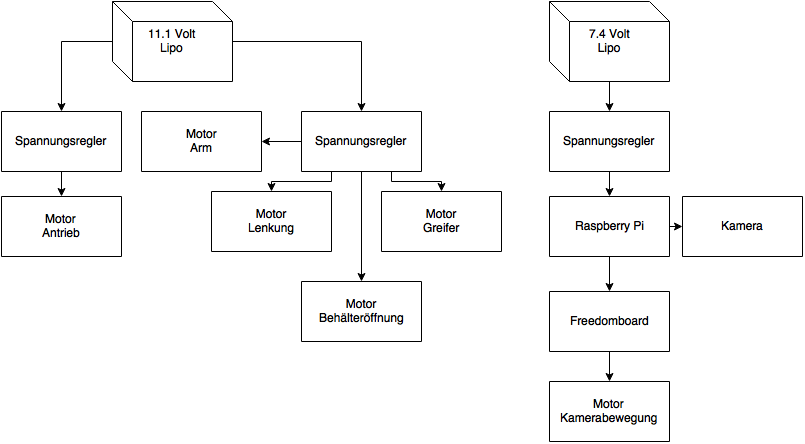
\includegraphics[width=0.8\textwidth]{03_Loesungskonzept/pictures/speisung.png}
\caption{Aufteilung der Akkumulatoren}	
\end{figure}
\textbf{Begründung}\\[0.2cm]
Die Entscheidung wird damit begründet, dass Lithium-Polymer-Akkumulatoren in einem vielfältigen Sortiment erhältlich sind und damit eine grosse Flexibilität bei der Auswahl ermöglichen. Somit würde sich auch die Suche nach einem Ersatz bei allfälligen Änderungen vereinfachen. Ausserdem weisen LiPos, im Vergleich zu anderen Akkumulatoren, eine wesentlich kompaktere Bauform auf, was entscheidend für die Auswahl war. \\[0.2cm]
\textbf{Berechnungen}\\[0.2cm]
Leistungsberechnungen:
\begin{itemize}
\item Servomotor für die Lenkung:
\[
P=2\cdot \pi\cdot N\cdot M \to 2\cdot \pi\cdot 0.92\frac{U}{sec}\cdot 0.65Nm = 3.76W
\]
\item Servomotoren für Kamerabewegung und Greifer:
\[
P=2\cdot \pi\cdot N\cdot M \to 2\cdot \pi\cdot 0.72\frac{U}{sec}\cdot 0.18Nm = 0.81W
\]
\item Servomotor für den Greiferarm:
\[
P=2\cdot \pi\cdot N\cdot M \to 2\cdot \pi\cdot 1.14\frac{U}{sec}\cdot 0.32Nm = 2.5W
\]
\item DC-Motor für den Antrieb:
\[
P=2\cdot \pi\cdot N\cdot M \to 2\cdot \pi\cdot 5.258\frac{U}{sec}\cdot 2.23Nm = 73.98W
\]
\item DC-Motor für die Behälteröffnung:
\[
P=2\cdot \pi\cdot N\cdot M \to 2\cdot \pi\cdot 16.6\frac{U}{sec}\cdot 0.028Nm = 2.9W
\]
\end{itemize}
\newpage
Kapazitätenberechnungen:
\begin{itemize}
\item DC-Motor für den Antrieb:
\[
\frac{P\cdot t}{U} \to \frac{73.98W\cdot0.25h}{12V}= 1.54 Ah
\]
\item DC-Motor für die Behälteröffnung:
\[
\frac{P\cdot t}{U} \to \frac{2.9W\cdot0.25h}{4.8V}= 0.15 Ah
\]
\item Servomotor für die Lenkung:
\[
\frac{P\cdot t}{U} \to \frac{3.76W\cdot0.25h}{4.8V}= 0.19 Ah
\]
\item Servomotor für den Greiferarm:
\[
\frac{P\cdot t}{U} \to \frac{2.5W\cdot0.25h}{4.8V}= 0.13 Ah
\]
\item Servomotoren für Kamerabewegung und Greifer:
\[
\frac{P\cdot t}{U} \to \frac{0.81W\cdot0.25h}{4.8V}= 0.04 Ah
\]
\item Mini-Computer:
\[
I\cdot t \to 2A*0.25h = 0.5 Ah
\]
\item Benötigte Kapazität für den 11.1 Volt Akkumulator:
\[
1.54Ah+0.15Ah+0.19Ah+0.13Ah+0.04Ah = 2.05Ah
\]
\item Benötigte Kapazität für den 7.4 Volt Akkumulator:
\[
0.5Ah
\]
\end{itemize}
\subsubsection{Akkuüberwachung Schwellwertberechnung}
Damit die LiPo-Akkumulatoren nicht zerstört werden, muss sichergestellt werden das diese nicht tief entladen werden. Dies wird über das Freedomboard gelöst. Die Akkuspannung wird über einen Analog - Digitalwandler eingelesen. Wenn die Akkuspannung einen gewissen Wert unterschreiten, werden die Verbraucher an den Akkus "abgeschaltet". Eine Lipozelle sollte die Zellenspannung von 3.7V nicht unterschreiten. Im Normalfall sollten alle Zellen einzeln überwacht werden, dies ist jedoch im Rahmen dieses Prototypen nicht angemessen. Als Kompromiss wird gesamte Ausgangsspannung gemessen. Das heisst zwei beziehungsweise drei Zellen in Serie (je nach Akku).\\
Das Freedomboard kann nur Spannungen bis 3.3V einlesen. Daher ist ein Spannungsteiler nötig. Damit dieser Wert sicher nicht überschritten wird, wird mit einer maximal zulässigen Spannung von 3V gerechnet. Für UAkku wurde 13V gewählt, damit der AD-Wandler sicher nie 3V erreicht.\\
Für den 11.1V Akku:
\[	U_Akku/U_Frd=R1/R2\]
\[	13V/3V=4.33=g\]
Gewählt:
\[	R2=10k R1=R2*4.33=43kOhm\]
Der Abschaltwert des drei Zellen Akkus ist 3.7V * 3 = 11.1V.
Nach dem Spannungswandler entspricht dies einer Spannung von \[Uin/g=11.1V*10kOhm/(10kOhm+43kOhm)=2.075V\]
3.3V enspricht 65'535. Somit entspricht eine Spannung von 2.075V einem eingelesenen Spannungswert von 41592. Falls dieser Wert über längere (wenige Sekunden) unterschritten wird, wird eine Nachricht an das Raspberry gesendet und das System heruntergefahren.

Für den 7.1V (logik) Akku wurde mit einer maximale Spannung von 8.5V gerechnet:
\[	U_Akku/U_Frd=R1/R2\]
\[	8.5V/3V=2.83\]
Gewählt:
\[	R2=10k R1=R2*2.83=28.3kOhm\]
Für UAkku wurde 7.4V als Abschaltwert gewählt.\\
7.4V nach dem Spannungswandler entspricht einer Spannung von \[Uin/g=7.4V*10kOhm/(10kOhm + 28.3kOhm)=1.947\]
3.3V enspricht 65'535. Somit entspricht eine Spannung von 1.974V einem eingelesenen Spannungswert von 38673. Dieser Wert musste angepasst werden, da der Akku zu früh abschaltete, da unter Last die Akkuspannung kurzzeitig sinkt. Ausgehend von dem gemessenen Wert von 32158 und einer Akkuspannung von 7.55V wurde der neue Wert von 31513 berechnet.
\\[0.2cm]
\textbf{Vergleich Konzept und Umsetzung}\\[0.2cm]
Die Akkuüberwachung konnte einfacher realisiert werden, als es im Pren1 konzipiert war. Dies deshalb, weil bei der Energieversorung auf eine galvanische Trennung der beiden Akkumulatoren verzichtet wurde. Dies ermöglichte das direkte einlesen des Spannungswertes über einen Spannungsteiler. Geplant war ursprünglich eine Vergleicherschaltung mit einem Operationsverstärker für den 11.1V Akkumulator. Diese Vereinfachung war auch sicher ein Grund auf die galvanische Trennung zu verzichten.

% !TEX root = ../Dokumentation.tex
\subsection{Elektronisches Layout}
Damit über den Mikrocontroller auf die einzelnen elektrischen Komponenten zugegriffen und mit ihnen kommuniziert werden kann, werden diese miteinander verbunden. Dazu werden sie auf eine Leiterplatte geführt welche auf den MCU gesteckt wird.
\\[0.2cm]

\textbf{PCB-Schaltung}\\[0.2cm]
Für die Leiterplatte wurde eine entsprechende Schaltung entworfen, die das Zusammenspiel der elektrischen Hardware ermöglicht. Dabei waren die technischen Spezifikationen der Teile ausschlaggebend für den Entwurf.
So musste beispielsweise gewährleistet werden, dass  keine zu hohen Spannungen auf den Mikrocontroller oder auf andere Komponente geführt werden. Für die Spannungsüberwachung der Akkumulatoren, wurde daher ein Spannungsteiler eingebaut. Mit diesem wird nicht das ganze Potential über den Mikrocontroller geführt, sondern nur ein Wert im vetragbaren Bereich. Bei den Motoren hingegen, wurden DC/DC-Wandler eingesetzt um die Spannung möglichst konstant auf 5V zu halten.
Die Schaltung wurde mithilfe des Altium Designer entworfen und das komplette Schema befindet sich im Anhang.
\\[0.2cm]

\textbf{PCB-Layout}
\\[0.2cm]
% !TEX root = ../Dokumentation.tex
\subsection{Intelligente Systeme}
\subsubsection{Softwarekonzept}
\textbf{Funktionsbeschrieb}\\[0.2cm]
Das Softwarekonzept basiert auf dem MVC\footnote{MVC = Model-View-Control}-Prinzip, wobei sich die View auf einen reinen Debug-Zweck beschränkt. Dementsprechend soll die View über eine Schnittstelle nach aussen verfügbar gestaltet werden, um auf dem Notebook entsprechende Debug-Komponenten betreiben zu können. Ebenfalls über Methoden nach aussen offengelegt, sollen die Regelungsparameter zur Laufzeit angepasst werden können. Im produktiven Betrieb ist diese Schnittstelle gemäss Aufgabenstellung geschlossen. Dabei hat der Controller alle Subprozesse sowie die Schnittstelle zur Hardwaresteuerung, via Mikrocontroller-Board realisiert, unter Kontrolle. Die parallel laufenden Subprozesse sind:
\begin{itemize}
\item Bilderzeugung,
\item Objekterkennung und
\item Fahrbahnerkennung.
\end{itemize}
\begin{figure}[H]
	\centering
	\includegraphics[width=0.8\textwidth]{03_Loesungskonzept/pictures/grobablauf.png}
	\caption{Aktivitätendiagramm Grobablauf}
\end{figure}
Der Zustand des Fahrzeuges wird im Model gespeichert und steht allen Prozessen zur Verfügung. Die Datenstruktur ist dabei so aufgebaut, dass keine Zugriffskonflikte entstehen sollten.\\
Der Controller behandelt alle Anweisungen der Prozesse. Meldet beispielsweise die Objekterkennung einen Container, hat dieser Priorität vor dem normalen Fahren und das Mikrocontroller-Board erhält die entsprechenden Anweisungen.\\[0.2cm]
\textbf{Komponentenbeschrieb}\\[0.2cm]
Umgesetzt wird das Konzept auf dem Minicomputer in C++. Dabei werden die zuvor beschriebenen Prozesse als eigene Threads realisiert. Um eine hohe Softwarequalität sicherzustellen, soll möglichst nach TDD\footnote{TDD = Test Driven Developement} gearbeitet werden. Für die automatisierten Tests werden die Open-Source-Pakete Google-Test und Google-Mock verwendet, welche in C++ realisiert und optimiert sind und sich direkt in das Projekt integrieren lassen.\\
Das Mikrocontroller-Board wird aus Effizienzgründen mit der Programmiersprache C programmiert.\\[0.2cm]
\textbf{Begründung}\\[0.2cm]
Der geplante Minicomputer verfügt über einen Vierkernprozessor, weswegen eine Parallelisierung zwingend notwendig wird, um diesen Prozessor auch vollumfänglich nutzen zu können. Bei der Programmiersprache ist C++ aufgrund der Performance und der einfachen Kopplung an C gewählt worden. Zudem sind keine Zusatztools wie virtuelle Maschinen notwendig. Die verwendete Bildverarbeitungssoftware OpenCV ist ebenfalls in C++ entwickelt und somit direkt nutzbar.\\
TDD soll sicherstellen, dass vor allem bei kurzfristigen Änderungen keine unerwünschten Nebeneffekte entstehen und jederzeit sichergestellt ist, dass die Software wunschgemäss läuft.
%***************************
\subsubsection{Mini-Computer}
\textbf{Funktionsbeschrieb}\\[0.2cm]
Der Mini-Computer beinhaltet die Logik- und Ablaufsteuerung, nimmt Bilder von der Kamera entgegen und verarbeitet diese um Container zu orten und in der Mitte der Fahrbahn zu bleiben. Die Lenkkorrektur und weitere Befehle zur Steuerung der Mechanik werden via USB Schnittstelle an das Mikrocontroller-Board weitergeleitet.\\[0.2cm]
\textbf{Komponentenbeschrieb}
\begin{figure}[H]
	\centering
	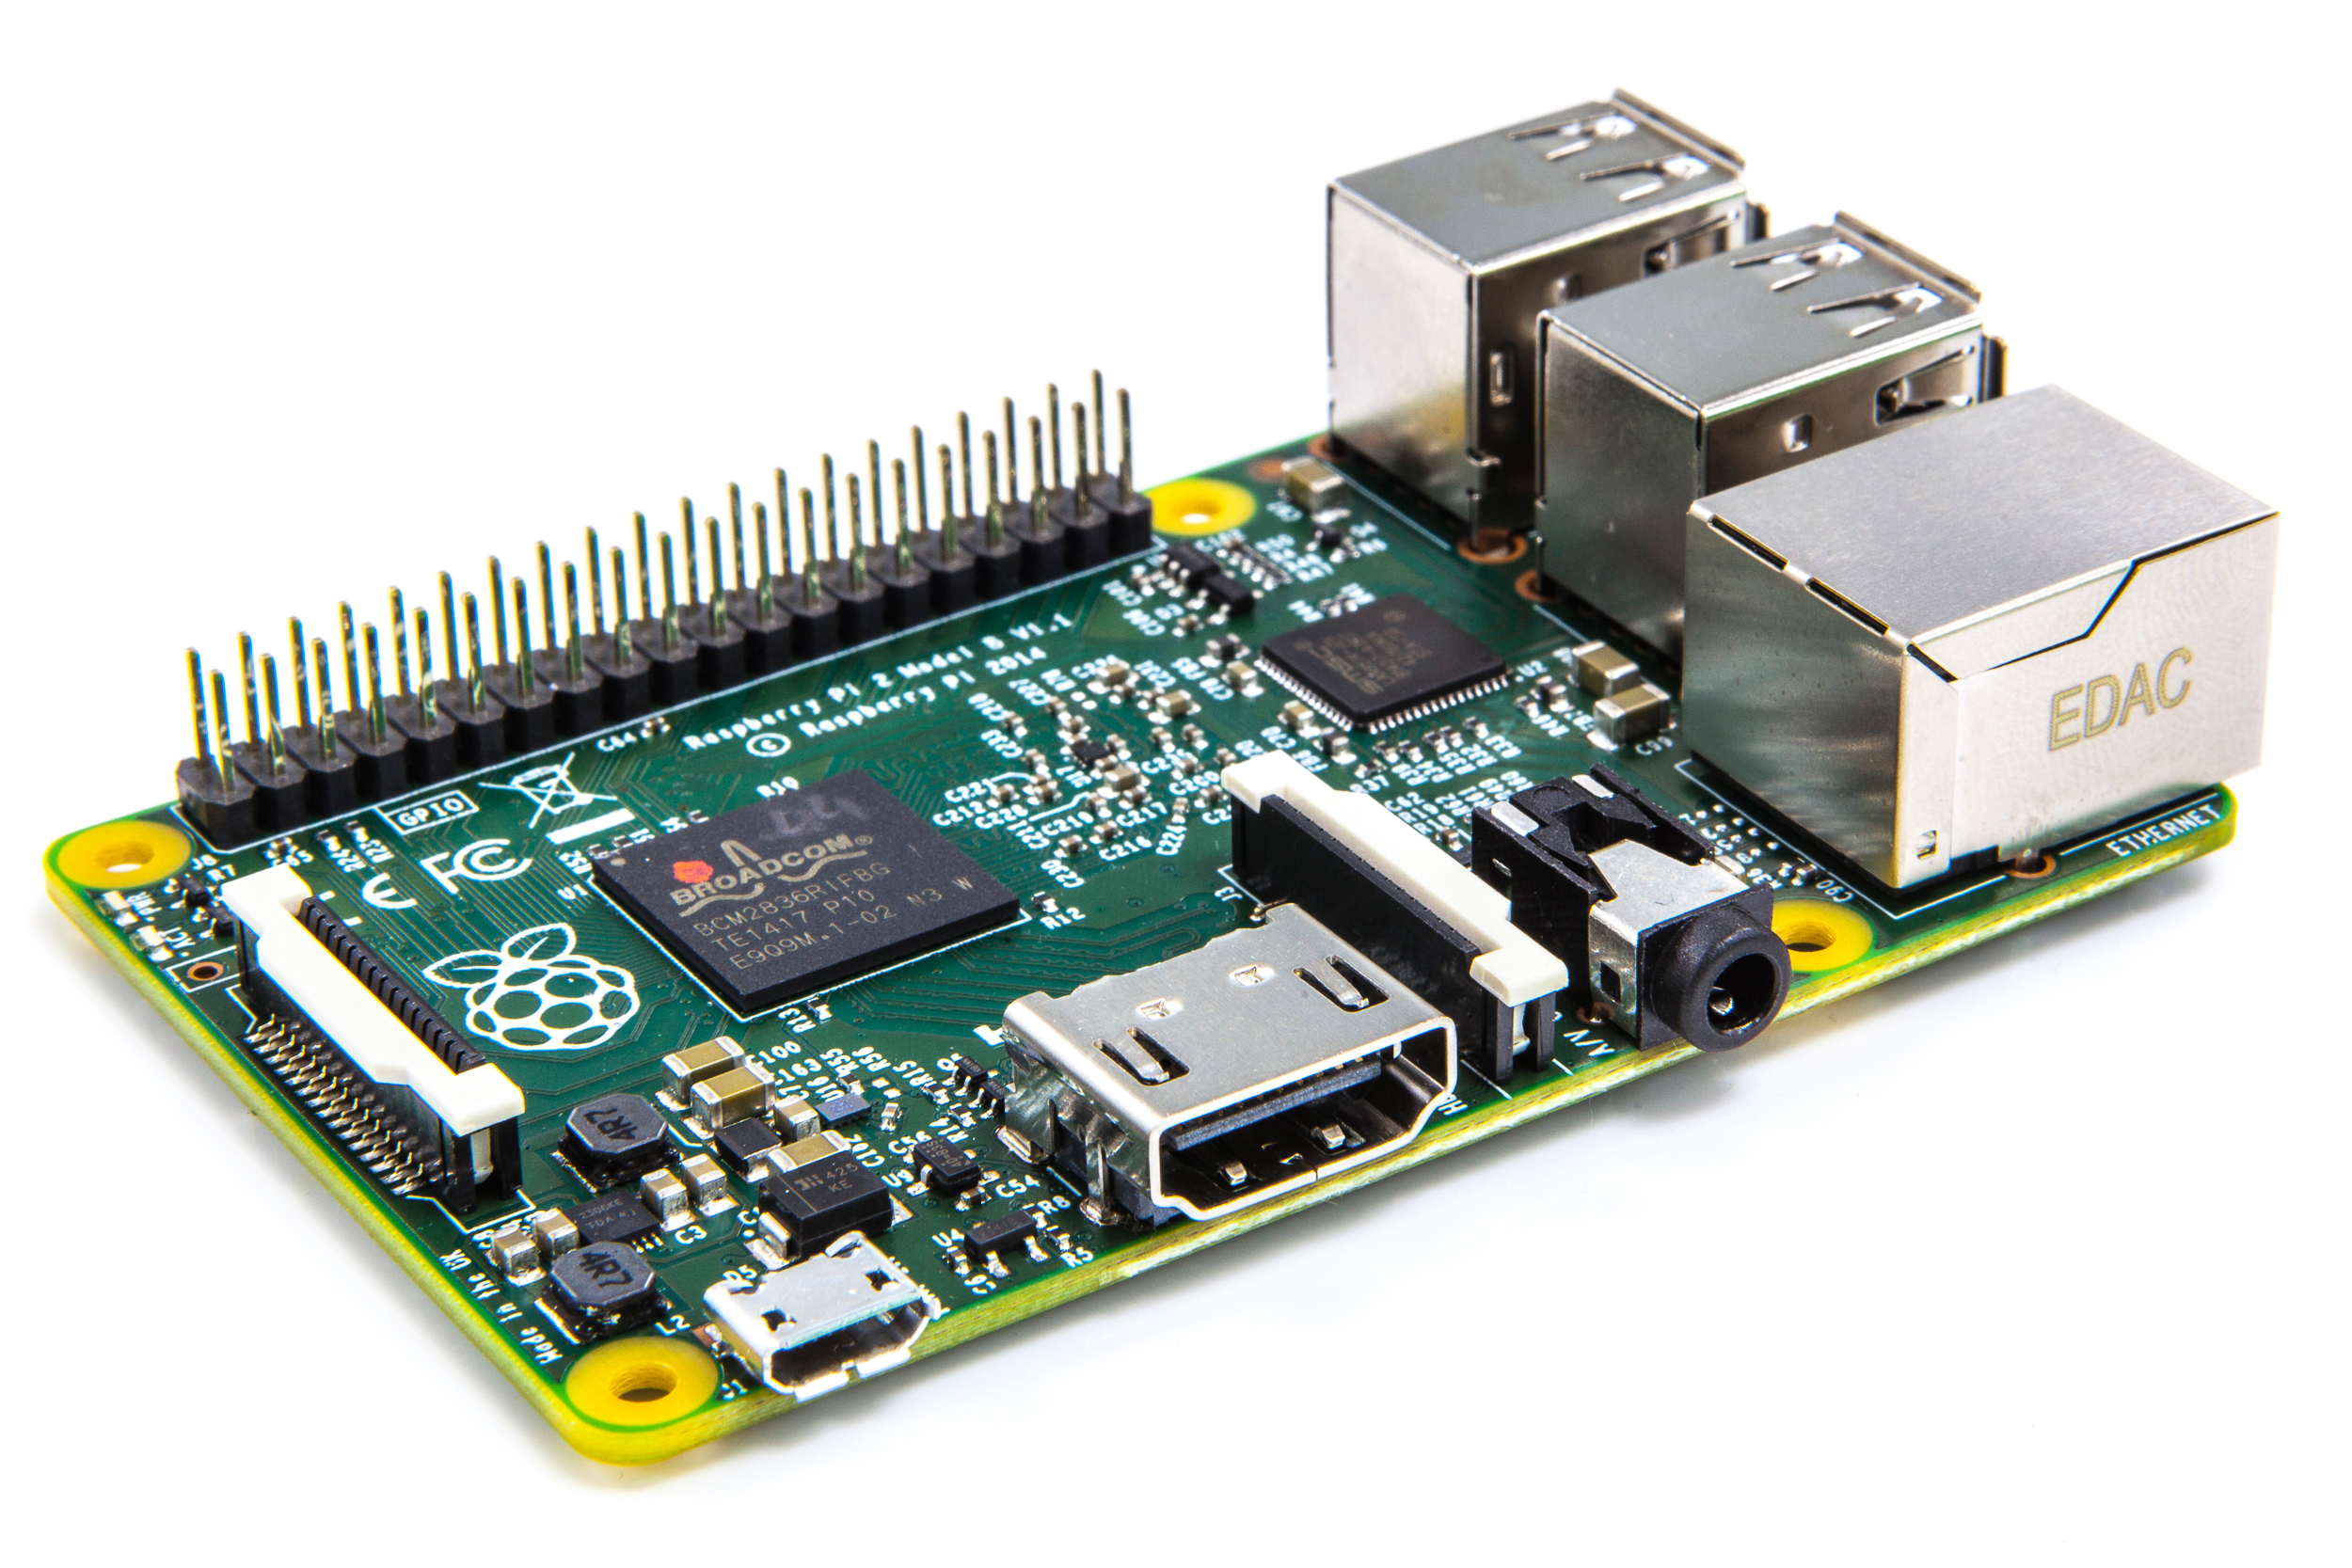
\includegraphics[width=0.5\textwidth]{03_Loesungskonzept/pictures/raspberrypi2.png}
	\caption{Raspberry Pi2 Model B (Quelle:http://pcworld.com/)}
\end{figure}
Das Raspberry Pi2 bietet mit einem 900MHz Quadcore Prozessor, einem eigenem Grafikchip und 1GB Ram viel Leistung und ist ideal geeignet.\\[0.2cm]
\textbf{Begründung}\\[0.2cm]
Dem Team war von Anfang an klar, dass die Bildverarbeitung viele Ressourcen verbrauchen wird. Gleichzeitig darf der Energieverbrauch die Kapazität eines Akkus nicht übersteigen. Das Raspberry Pi2 besitzt genügend Leistung und ist trotzdem sparsam. Mit einem Quadcore und 1GB RAM ist es ausreichend leistungsfähig um Bilder zeitig zu verarbeiten. Zusätzlich ist es einfach zu verwalten und zu bedienen, da es über ein eigenes Betriebssystem verfügt.
%***************************
\subsubsection{Mikrocontroller-Board}
\textbf{Funktionsbeschrieb}\\[0.2cm]
Das Mikrocontrollerboard bildet die Schnittstelle zwischen der Hardware (Motoren und Sensoren) und dem Minicomputer. Das Mikrocontrollerboard übernimmt die Ansteuerung und Auswertung der einzelnen Komponenten und stellt die verarbeiteten Informationen dem Minicomputer über eine Schnittstelle zur Verfügung.\\[0.2cm]
\newpage
\textbf{Komponentenbeschrieb}
\begin{figure}[H]
	\centering
	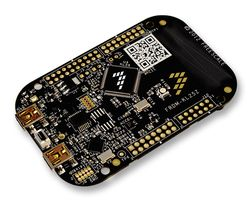
\includegraphics[width=0.5\textwidth]{03_Loesungskonzept/pictures/freedomboard.png}
	\caption{Freedomboard KL25 von Freescale (Quelle:http://ch.farnell.com/)}
	%http://ch.farnell.com/productimages/standard/de_DE/freescalesemiconductor-frdm-kl25z-40.jpg
\end{figure}
Als Mikrocontrollersystem wurde das Freedomboard KL25Z von Freescale ausgewählt. Das Entwicklungsgsboard bietet vieles, wie ausreichend I/O's, AD Wandler und Timerausgänge. Das Board wird mit der Programmiersprache C programmiert.\\[0.2cm]
\textbf{Begründung}\\[0.2cm]
Das Board überzeugt durch eine gute Rechenperformance zu einem kleinen Preis. Das Hauptargument für das Freedomboard ist die einfache Programmierung. Für viele Komponenten wie Servos oder Ultraschalsensoren steht ein Tool namens ProcessorExpert zu Verfügung. Dieses Tool ermöglicht eine relativ einfache Anbindung solcher Komponenten. Dies spart sehr viel Entwicklungsaufwand.
Das Freedomboard hat sich gegen das Tinkerforgesystem durchgesetzt. Der Hauptgrund ist die Flexibilität des Freedomboards gegenüber dem Tinkerforgesystem. Dieses ist sehr einfach zu bedienen solange alle Komponenten von Tinkerforge zur Verfügung gestellt werden. Fehlt aber ein Modul wird es sehr schnell kompliziert. Beim Freedomboard ist der Aufwand für eine Komponente etwas höher, dafür können die meisten Systeme angeschlossen werden.\\[0.2cm]
\textbf{Testergebnisse}\\[0.2cm]
Das Freedomboard wurde als Funktionsmuster bereits in Betrieb genommen. Es hat sich gezeigt, dass die Anbindung der Komponenten tatsächlich sehr einfach ist. Es wurden bereits ein Ultraschallsensor, mehrere Servos, eine UART Kommunikation und ein Infrarotsensor angebunden. Das System lieferte dabei sehr vielversprechende Ergebnisse.\\[0.2cm]
\textbf{Software Grundaufbau}\\[0.2cm]
Das Tool ProcessorExpert bietet eine Komponente FreeRTOS an. Das ist ein Betriebssystem, welches das Programmieren sehr vereinfacht. Damit können verschiedene Tasks definiert werden und quasi parallel ausgeführt werden. Die Software wird damit geplant. Folgende Tasks sind geplant:
\begin{figure}[H]
	\centering
	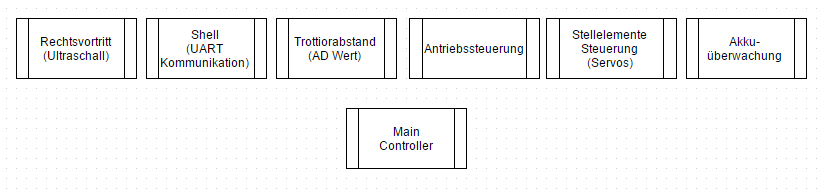
\includegraphics[width=0.9\textwidth]{03_Loesungskonzept/pictures/MC_Tasks.png}
	\caption{Übersicht MC Tasks}
\end{figure}
Die Implementierung der Tasks wird im Modul Produkteentwicklung zwei (PREN2) umgesetzt.
% !TEX root = ../Dokumentation.tex
\subsection{Bilderzeugung}
\textbf{Funktionsbeschrieb}\\[0.2cm]
Die Bilderzeugung stellt die Schnittstelle zur Kamera sicher und speichert die erzeugten Bilder fortlaufend in einer von OpenCV zu Verfügung gestellten Datenstruktur bereit. Dabei wird jeweils nur das aktuellste Bild der Kamera zu Verfügung gestellt.\\
Als Kamera kommt die Raspberry Pi CAM zum Einsatz (Abbildung \ref{fig:camera}), die über eine MIPI Schnittstelle direkt an den Minicomputer angeschlossen und Kostengünstig erworben werden kann. Das Bilformat lässt sich über den Open Source Treiber einstellen, was zu einer Performanceverbesserung beiträgt. Der Winkel von 53° ist etwas knapp, daher wird die Kamera drehbar auf dem Fahrzeug montiert. Dies soll für die Kurvenfahrt sowie den Rechtsvortritt genutzt werden. Der Neigungswinkel der Kamera lässt sich ebenfalls einstellen, um die benötigte Flexibiltät der Sichtposition der Kamera sicherzustellen.
\begin{figure}[H]
\centering
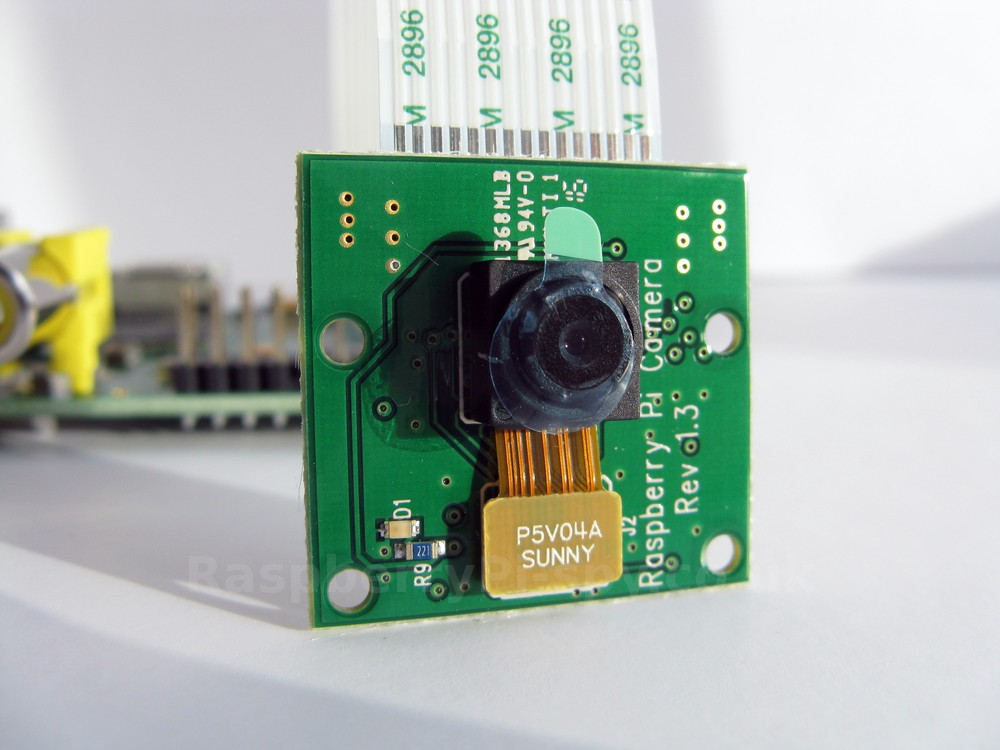
\includegraphics[width=0.6\textwidth]{03_Loesungskonzept/pictures/raspberry-pi-camera-module.jpg}
\caption{Raspberry Pi Kameramudul}
\label{fig:camera}
\end{figure}
\textbf{Komponentenbeschrieb}\\[0.2cm]
Die Bilderzeugung ist ein eigener als Thread realisierter Subprozess und liefert über die Methode \code{GetImage()} den Pointer auf das Bild zurück. Die verfügbare Datenstruktur ist dabei \code{cv::Mat} in Farbe mit einer Auflösung von 640x320 Pixel. Die verwendenden Prozesse können sich dann den Bildinhalt zeitgleich und unabhängig voneinander abgreifen und bedarfsgerecht weiterverarbeiten. Gestartet wird der Prozess automatisch bei der Objekterzeugung im Konstruktor und kann über die Methode \code{StopRecording()} angehalten werden, sobald das Ziel erreicht worden ist. Dem Konstruktor wird als Übergabeparameter der Pointer auf den \code{PrenController} mitgegeben, so dass im Störungsfall entsprechende Meldungen an den Controller übergeben werden können.\\[0.2cm]
\textbf{Begründung}\\[0.2cm]
Der beschrieene Lösungsansatz bietet den Vorteil, dass die Fahrbahnerkennung und die Objekterkennung, welche diesen Prozess benutzen, unabhängig voneinander ihre Weiterverarbeitung parallel durchführen können. So wird der Mehrkernprozessor des Minicomputers optimal genutzt. Weiter  sollte eine Synchronisation der \code{GetImage()}-Methode nicht notwendig sein, da das erzeugte Bild nicht verändert, sondern nur genutzt wird, was sich wiederum positiv auf die Performance auswirkt.\\[0.2cm]
\textbf{Testergebnisse}\\[0.2cm]
Anhand der Test mit dem Minicomputer und der entsprechenden Kamera werden ca 20-30 Frames pro Minute zu Verfügun gestellt. Die Bilder sind dabei in guter Qualität und mit wenig Glanzeffekten entstanden. Es könnte dennoch von Vorteil sein, den Glanz noch wegzufiltern um Störungen zu vermeiden.\\
Die parallelen Zugriffe haben sich in den Tests bewährt und konfliktfrei funktioniert.
% !TEX root = ../Dokumentation.tex
\subsection{Fahrbahnerkennung}
\textbf{Funktionsbeschrieb}\\
Die Fahrbahnerkennung soll primär mittels Kamera umgesetzt werden. Dazu werden Bilder aus dem zu Verfügung gestellten Bilderpool entnommen, mit OpenCV in Graustufen umgewandelt und anschliessend einer Kantenanalyse unterzogen. Dazu wird ein eigener Algorithmus verwendet, der jeweils eine Bildzeile als Graph einer Funktion $y = f(x)$ angeschaut, wobei $x$ der Pixelkoordinate der Spalte und $y$ dem Graustufenwert des Pixels entspricht.\\
Anhand der vorhandenen Informationen kann die Fahrbahn und demzufolge während der Fahrt der Korrekturvektor ermittelt werden. Die Korrektur selber soll mittels PID-Regelung realisiert werden, um eine ruhige Fahrt zu erreichen.\\
\textbf{Komponentenbeschrieb}
\begin{figure}[h!]%Position festigen
\centering
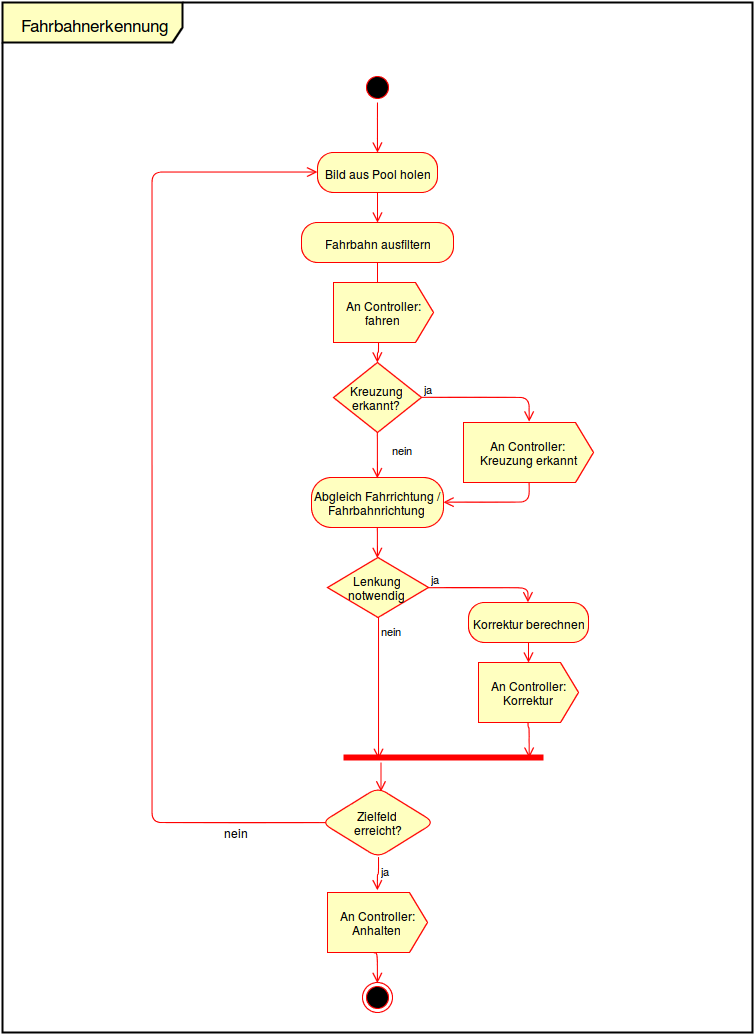
\includegraphics[width=0.6\textwidth]{03_Loesungskonzept/pictures/Fahrbahnerkennung.png}
\caption{Aktivitätendiagramm Fahrbahnerkennung}
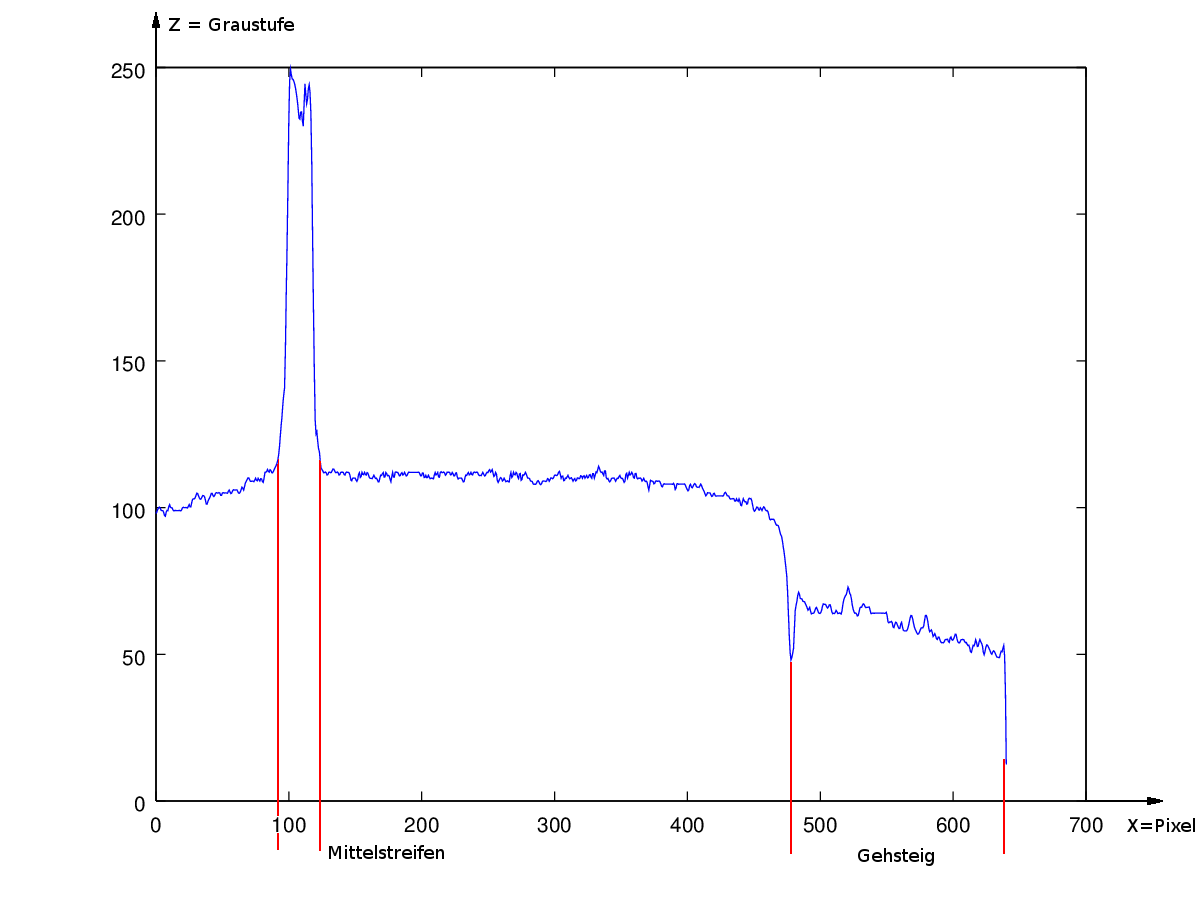
\includegraphics[width=0.6\textwidth]{03_Loesungskonzept/pictures/graphPicture.png}
\caption{Graph der Graustufenwerte einer Bildzeile}
\label{fig:grayscale}
\end{figure}\\
Die Fahrbahnerkennung wird als eigener Thread auf dem Raspberry Pi realisiert und in C++ objektorientiert umgesetzt. Für die Kantenerkennung wird jede Zeile eines Bildes als Funktion angeschaut und falls die Änderungsrate den Filterwert überschreitet eine Kante erkannt (Abbildung). \\
Im Anschluss wird im unteren Bereich des Bildes von innen nach aussen die Fahrbahn gesucht. Dazu werden jeweils in beide Richtungen die ersten Kanten gesucht, über mehrere Punkte fixiert und danach alle übrigen Kanten entfernt.\\
Da die Fahrbahn keine Sprunghaften Änderungen aufweisen kann, wird die Kantendetektierte Matrix von unten nach oben durchgesehen und alle Kanten, die in $x$ - Richtung eine zu grosse Abweichung von der erkannten Fahrbahn aufweisen entfernt, so dass nur noch die rechte und linke Fahrbahnbegrenzung übrig bleibt. Die Mitte zwischen diesen Kanten wird anschliessend in die Zielspur umgewandelt.\\
\textbf{Begründung}\\
Mit der beschriebenen Vorgehensweise kann der Aufwand pro Bild gegenüber OpenCV deutlich reduziert werden, da die Operationen ausschliesslich für die Fahrbahnerkennung erstellt werden. Die Tests haben die Realisierbarkeit dieser Vorgehensweise als machbar und fexibel aufgezeigt.\\
\textbf{Berechnungen}\\
Komplexität des Algorithmus, jedes Bild wird als eine $n\times{m}$ Matrix $M$ betrachtet wobei $n=x$ = Spaltenzahl und $m$ = Zeilenzahl. Die Resultate der Kantenerkennung werden in einer zweiten $n\times{m}$ Matrix $M_1$ gespeichert, welche für die weiteren Berechnungen verwendet wird.
\begin{itemize}
\item Iteration für Kantenerkennung:
\[
n \cdot m \leq n \cdot n \text{ wenn } n\geq m \rightarrow \mathcal{O}(n^2) \text{ mit den Zeugen }C=1 \text{ und } k = m
\]
\item Iteration für Kantenfindung Fahrbahn:
\[
10m \leq 10n  \text{ wenn } n\geq m \rightarrow \mathcal{O}(n) \text{ mit den Zeugen }C=10 \text{ und } k = m
\]
\item Iteration für Fahrbahnausfilterung und das Erzeugen der Sollspur:
\[
n \cdot m \leq n \cdot n \text{ wenn } n\geq m \rightarrow \mathcal{O}(n^2) \text{ mit den Zeugen }C=1 \text{ und } k = m
\]
\item Zusammengezogene Schätzung der Komplexität:
\begin{align*}
2(n^2) + 10n &\leq 2n^2 + 10n^2 \text{ wenn } n\geq 1\\
             &= 12n^2\\
             &\rightarrow \mathcal{O}(n^2) \text{ mit den Zeugen }C=12 \text{ und } k = m
\end{align*}
\end{itemize}
Formeln für die Berechnungen:
\begin{itemize}
\item Kantenfindung $h=$ Grenzwert für die Änderungsrate um eine Kante zu ermitteln und $y_1$ der Wert des Pixels in der Zielmatrix $M_1$:
\[
y = f(x) = \text{ Graustufen des Pixels }0 \leq y \leq 255
\]
$x:=1 \text{ to } n-2 \text{ step } 1$\\ 
$\textbf{if } f(x+2)-f(x) \geq h \textbf{ then } y_1 = 255 \textbf{ else } y_1 = 0$\\
\end{itemize}
\textbf{Testergebnisse}\\
% !TEX root = ../Dokumentation.tex
\subsection{Objekterkennung}
Die Objekterkennung hat das Ziel die richtigen Objekte zu erkennen und das genaue Positionieren des Fahrzeuges zu ermöglichen. Dabei wird die Containererkennung in zwei Teilaufgaben aufgeteilt. Die Objekterkennung grob ist für die Erkennung der richtigen Objekte mittels Farb- und Formerkennung zuständig. Die Objekterkennung präzise ist für das Positionieren des Fahrzeuges notwendig. Diese zwei Teilaufgaben werden separat angeschaut.
%
\subsubsection{Objekterkennung grob}
Die Aufgabe der Objekterkennung grob ist es, die aufzuladenden Container, kreuzenden Fahrzeuge und das Entleerungsbecken zu erkennen. Sobald ein ein solches Objekt erkannt wird, wird der zentrale Controller darüber informiert, damit die Informationen an die Objekterkennung präzise weitergegeben werden können.
\\[0.2cm]
\underline{\textbf{Container und Entleerungsbecken}}
\\[0.2cm]
\textbf{Funktionsbeschrieb}\\[0.2cm]
Bei der Container- und Entleerungsbeckenerkennung werden einerseits grüne und blaue Container und andererseits, im letzten Teil der Strecke, das Entleerungsbecken erkannt. Wird eines dieser Objekte erkannt, wird der Controller darüber informiert, damit sich das Fahrzeug auf das Auf- bzw. Abladen vorbereiten kann.
\\[0.2cm]
\textbf{Komponentenbeschrieb}\\[0.2cm]
Sobald die ersten Bilder mit der Kamera aufgenommen wurden, werden diese laufend aus dem Bilderpool abgefragt und untersucht. Dabei läuft die Erkennung von grünen und blauen Containern parallel ab. Erst sobald die Kreuzung zum zweiten Mal passiert wurde, wird auch nach dem Entleerungsbecken gesucht.
\begin{figure}[H]%Position festigen
\centering
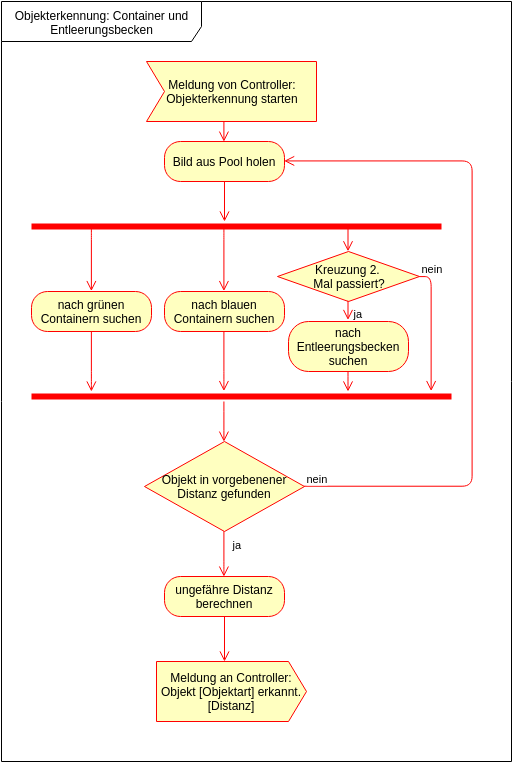
\includegraphics[width=0.6\textwidth]{03_Loesungskonzept/pictures/objekterkennung_containers.png}
\caption{Aktivitätendiagramm Obkjekterkennung: Container und Entleerungsbecken}
\label{fig:activityContainer}
\end{figure}
\flushleft
Die Erkennung läuft dabei immer gleich ab. Als erstes wird das Bild mit OpenCV nach der entsprechenden Farbe gefiltert. Sprich: Es wird nur nach Grün-, Blau- und Weisstönen gesucht. Anschliessend werden mit Hilfe einer Konturerkennung störende und falsche Objekte entfernt. Mit der Höhe dieser Objekte kann dann ausgerechnet werden, wie weit das Objekt  noch entfernt ist. Diese Distanzberechnung liefert nur ein ungefähres Ergebnis. Ist das Objekt zu weit entfernt, wird der zentrale Controller nicht informiert. Ansonsten wird eine Meldung an den Controller gesendet, welche die Objektart und Distanz enthält.
\\[0.2cm]
\textbf{Begründung}\\[0.2cm]
Da der Blickwinkel auf die Container durch die Kurven variieren kann, wäre es wenig sinnvoll die Konturerkennung vor der Farberkennung durchzuführen. Es bestehen zu viele Möglichkeiten, dass ein störendes Objekt als Container oder Entleerungsbecken identifiert werden könnte. Dadurch, dass zuerst nach Farben gefiltert wird, können bereits viele falsche Objekte ausgeschlossen werden. \\
OpenCV stellt Methoden zur Verfügung, mit welcher ein ganzer Bereich mit Farbwerten im HSV-Format angegeben werden kann. Das bedeutet, dass auch bei unterschiedlichen Lichtverhältnissen die Farbtöne korrekt erfasst werden können.
\\[0.2cm]
\textbf{Testergenisse} \\[0.2cm]
Die Containererkennung wurde bereits soweit getestet, dass grüne und blaue Container bis auf eine bewusst eingeschränkte Distanz erkannt werden. 
\begin{figure}[H]%Position festigen
\centering
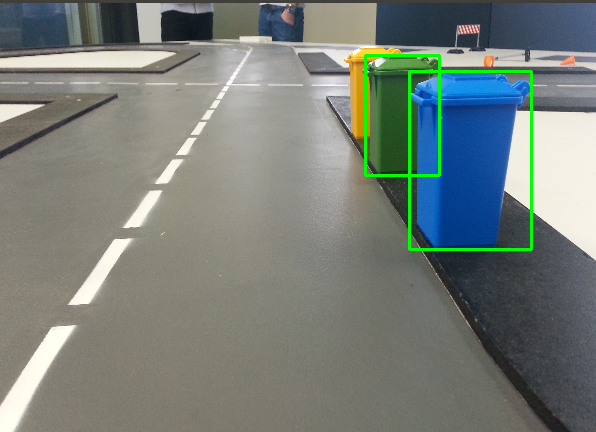
\includegraphics[width=0.6\textwidth]{03_Loesungskonzept/pictures/containererkennung_blau_gruen.png}
\caption{erfolgreicher Testversuch}
\label{fig:erfolgreicher Testversuch}
\end{figure}
\flushleft
Auch bei aufgenommenen Bildern, welche gleichfarbige Container mit unterschiedlichen Lichtverhältnissen zeigen, konnten die Container korrekt erkannt werden:
\begin{figure}[H]%Position festigen
\centering
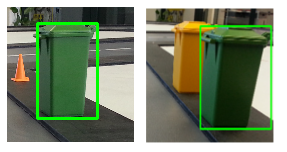
\includegraphics[width=0.6\textwidth]{03_Loesungskonzept/pictures/containererkennung_div_brightness.png}
\caption{unterschiedliche Helligkeiten}
\label{fig:unterschiedliche Helligkeiten}
\end{figure} \\
\flushleft
Bei den Testversuchen wurden jedoch auch Probleme und Risiken aufgedeckt. Falls zum Beispiel im Hintergrund ein Objekt steht, welches eine grüne oder blaue Farbe hat und die Masse einem Container entsprechen könnten, kann es zu einer Fehlerkennung kommen. Folgendes Bild zeigt einen solchen Fall:
\begin{figure}[H]%Position festigen
\centering
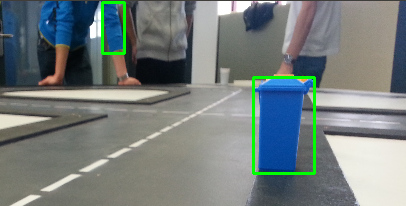
\includegraphics[width=0.6\textwidth]{03_Loesungskonzept/pictures/objekterkennung_blau_fehl.png}
\caption{fehlerhafter Testversuch}
\label{fig:fehlerhafter Testversuch}
\end{figure} \\
\flushleft
Um solche Fälle möglichst zu vermeiden wird versucht den abzusuchenden Bereich  einzuschränken, sodass nur solche Bildbereiche untersucht werden, wo sich auch wirklich ein Container befinden könnte. 
\\[0.2cm]
\underline{\textbf{Rechtsvortritt}}
\\[0.2cm]
\textbf{Funktionsbeschrieb}\\[0.2cm]
Falls sich an der Kreuzung ein gegnerisches Fahrzeug von rechts nähert, hat dieses gemäss Aufgabenstellung Vortritt. Die Objekterkennung muss ein solches Fahrzeug erkennen und den Controller darüber informieren, damit das Fahrzeug gestoppt wird.
\\[0.2cm]
\textbf{Komponentenbeschrieb}\\[0.2cm]
Sobald die Objekterkennung vom Controller informiert wird, dass das Fahrzeug gleich an der Kreuzung ankommen wird, wird Ausschau nach einem gegnerischen Fahrzeug auf der von rechtskommenden Spur gehalten. Wird ein Fahrzeug erkannt, wird dies dem Controller gemeldet. Der Vorgang wird wiederholt, bis das Fahrzeug nicht mehr im Bereich liegt. Sobald dies geschehen ist, wird wieder der Controller informiert, damit das Fahrzeug weiterfahren kann.
\begin{figure}[H]%Position festigen
\centering
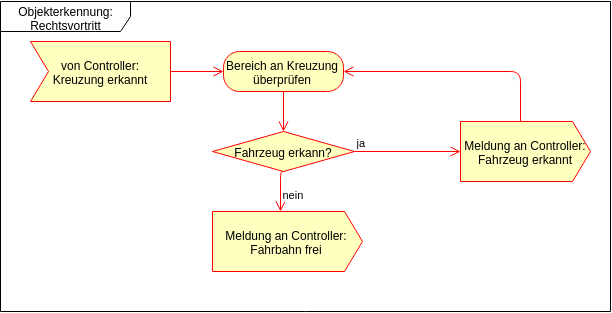
\includegraphics[width=0.8\textwidth]{03_Loesungskonzept/pictures/objekterkennung_rechtsvortritt.png}
\caption{Aktivitätendiagramm Obkjekterkennung: Rechtsvortritt}
\label{fig:activityRechtsvortritt}
\end{figure} \\
\flushleft
Da nicht nur angehalten werden muss, wenn ein gegenerisches Fahrzeug an der Kreuzun steht, sondern auch, wenn es sich von rechts nähert, muss der zu überprüfende Bereich eine gewisse Grösse haben. Der ungefähre Bereich, welcher abgesucht werden soll, ist in der folgenden Grafik markiert:
\begin{figure}[H]%Position festigen
\centering
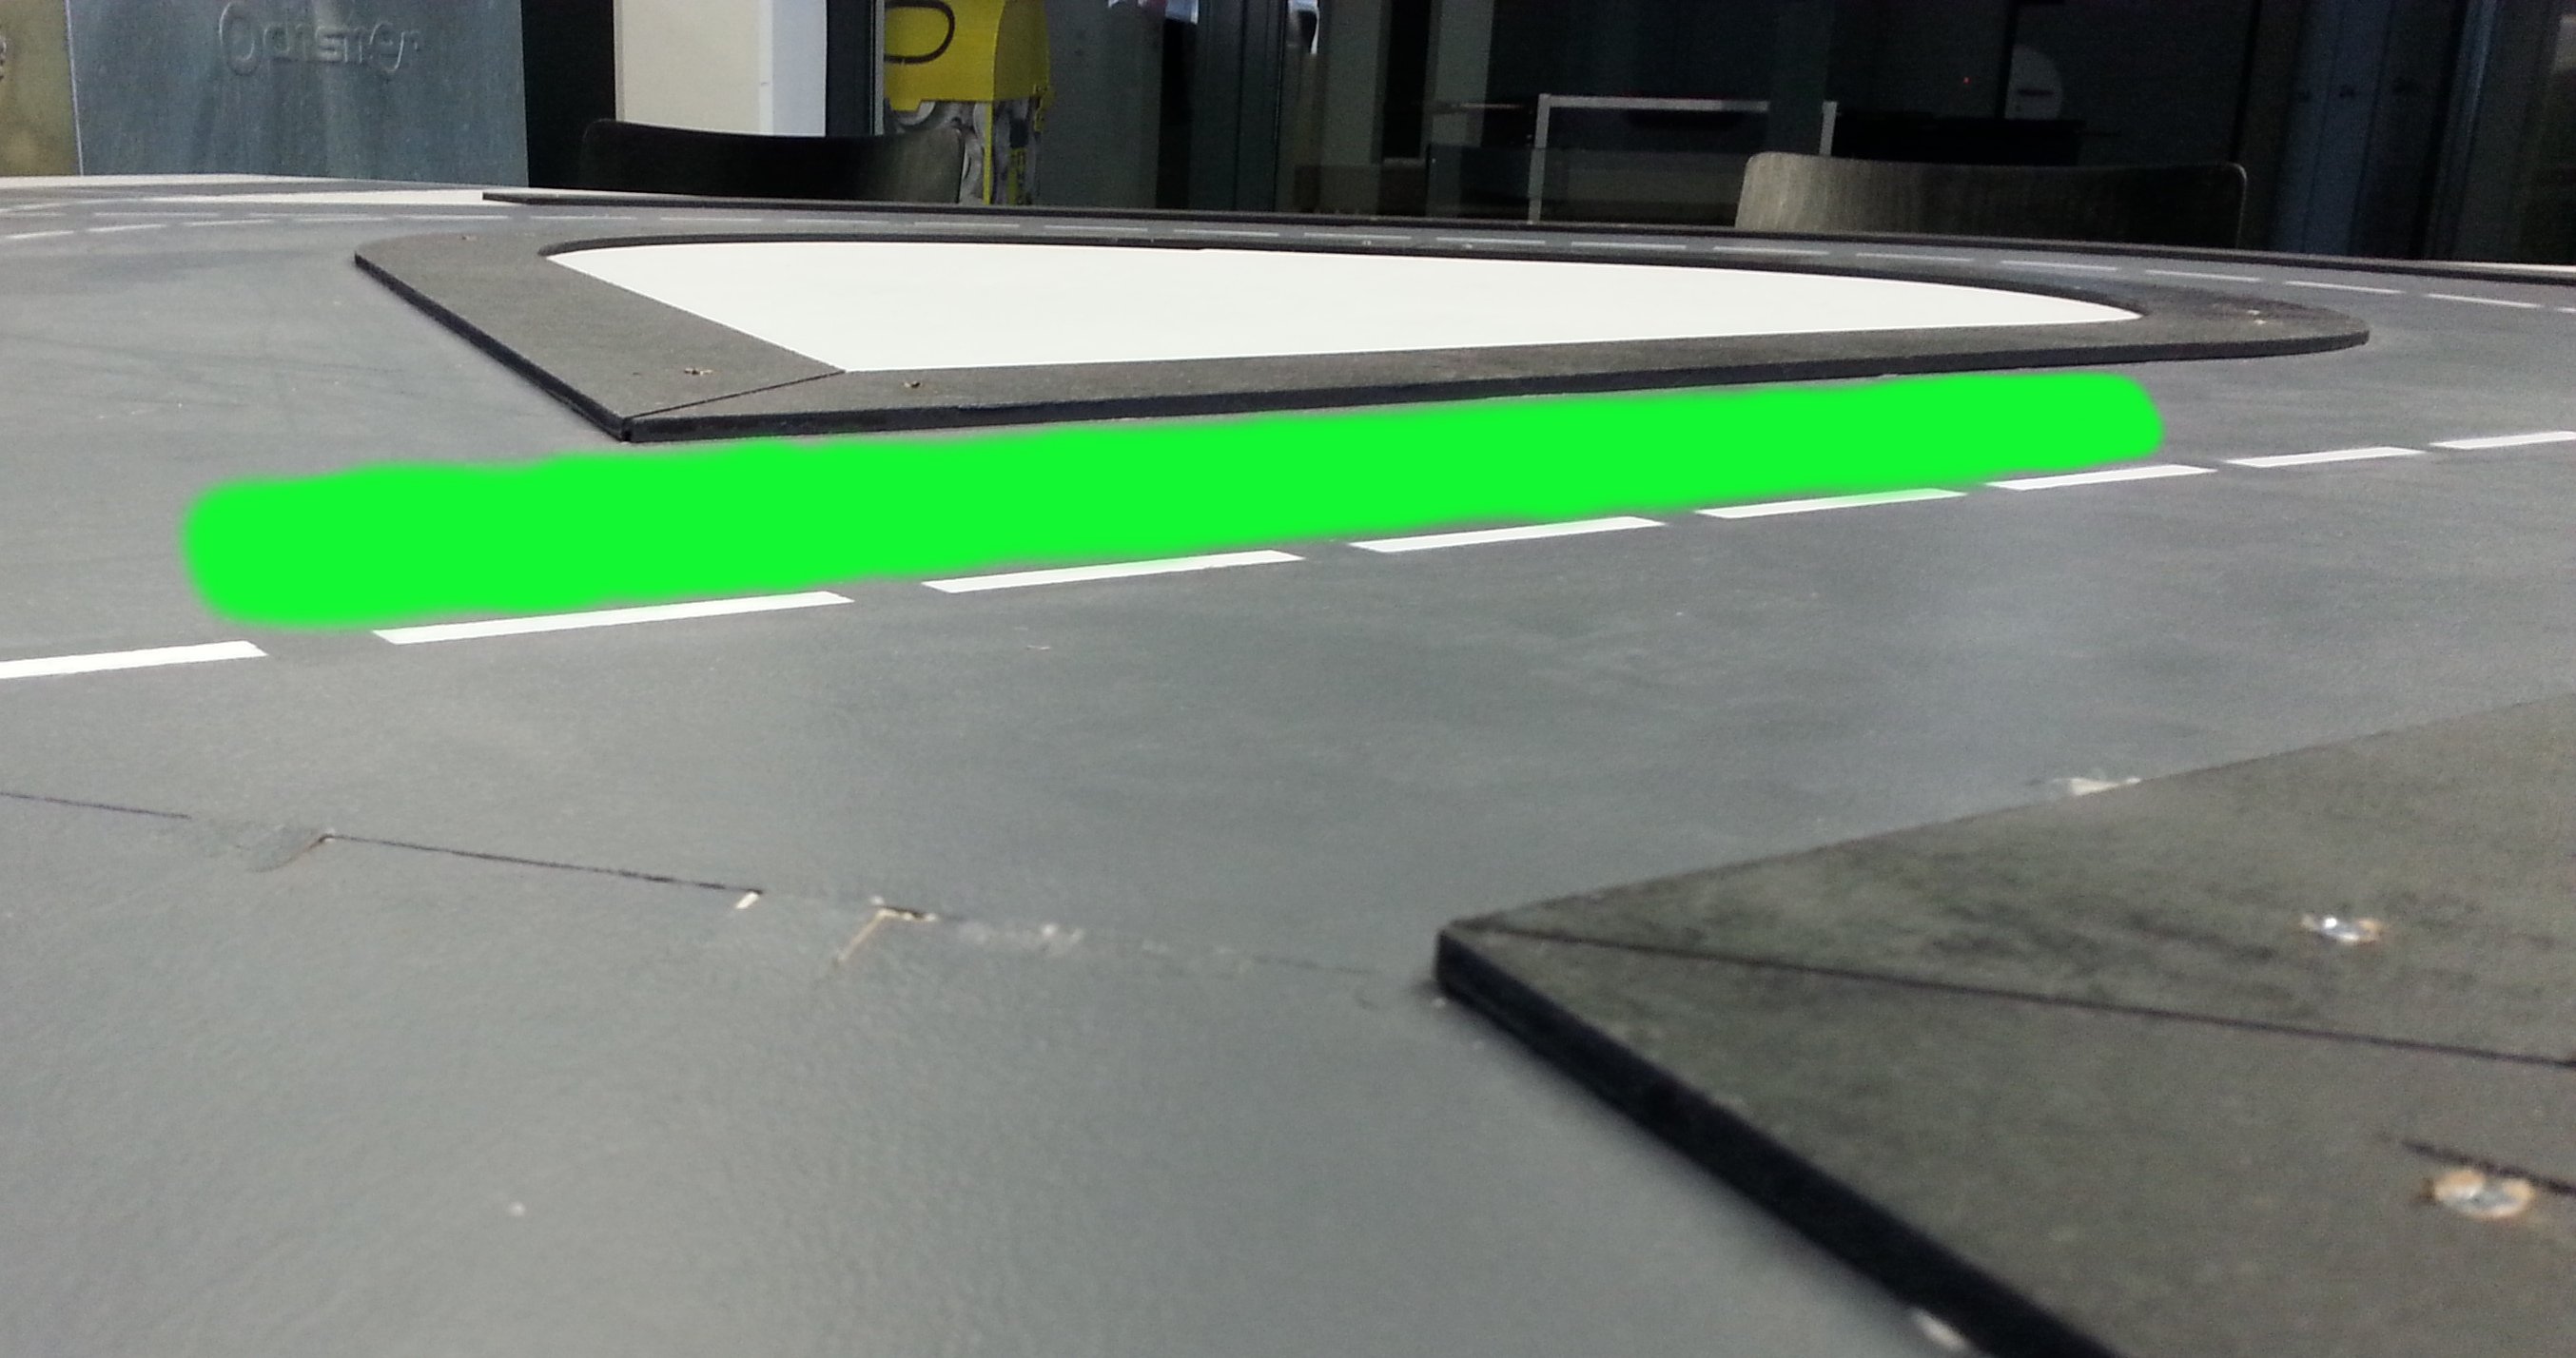
\includegraphics[width=0.8\textwidth]{03_Loesungskonzept/pictures/rechtsvortritt_bereich.jpg}
\caption{Abgedeckter Bereich beim Rechtsvortritt}
\label{fig:bereichRechtsvortritt}
\end{figure}
\\
\flushleft
\textbf{Begründung}\\[0.2cm]
Bei der Vortrittserkennung kann nicht nach Farben oder Konturen gesucht werden, da keine Angaben vorhanden sind, wie das gegnerische Fahrzeug aussieht. Daher ist es nötig, dass erkennt werden kann, ob ein definierter Strassenabschnitt verdeckt ist oder nicht. Falls der Abschnitt verdeckt ist, heisst das, dass sich ein Fahrzeug darauf befindet, welches Vortritt hat.
\subsubsection{Objekterkennung präzise}
\underline{\textbf{Containererkennung}}\\[0.2cm]
\textbf{Funktionsbeschrieb}\\[0.2cm]
Die präzise Containererkennung wird für das genaue Stoppen des Fahrzeuges gebraucht. Dieses Modul gibt den Trigger zum Anhalten.\\[0.2cm]
\textbf{Komponentenbeschrieb}\\[0.2cm]
Die Containererkennung wird mit Hilfe von Distanzsensoren realisiert. Dafür sind Infrarot Distanzmesser oder Infrarot Reflexkoppler vorgesehen. Diese werden auf der rechten Seite des Fahrzeuges befestigt. Sobald ein Objekt in der Nähe ist, ändert sich der Spannungswert, was einer Distanzänderung gleichkommt. 
\begin{figure} [H]
	\centering
	\includegraphics[width=0.35\textwidth]{03_Loesungskonzept/pictures/InfrarotContainererkennung.png}
	\caption{Beispielhafte Containererkennung mit einem Infrarotsensor}
\end{figure}
\flushleft
\textbf{Begründung}\\[0.2cm]
Die Positionierung mit einem Infrarotsensor ist die ideale Lösung. Sie ist einfach zu realisieren im Vergleich zu einer Kamera oder einem Farbesensor und präziserer als ein Ultraschallsensor.\\[0.2cm]
\textbf{Testergebnisse}\\[0.2cm]
Für die Ermittlung des besten Sensors wurde ein Ultraschall und Infrarotsensor als Funktionsmuster getestet. Der relativ grosse \glqq{Empfangswinkel}\grqq, welcher der Ultraschallsensor aufweist, ist in dieser Anwendung nicht gewollt. Der Infrarotsensor ist diesbezüglich besser. Dieser ist zwar lichtempfindlich, jedoch sollte dieses Problem gelöst werden können.\\[0.2cm]
%
\underline{\textbf{Rechtsvortritt}} \\[0.2cm]
\textbf{Funktionsbeschrieb}\\[0.2cm]
Die Rechtsvortritterkennung detailliert hat die Aufgabe das Fahrzeug vor einer Kollision zu Bewahren. Wenn rechts oder vor dem Fahrzeug etwas im Weg ist, soll das Fahrzeug anhalten.\\[0.2cm]
\textbf{Komponentenbeschrieb}\\[0.2cm]
\begin{figure} [H]
	\centering
	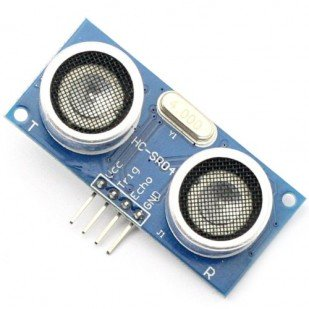
\includegraphics[width=0.25\textwidth]{03_Loesungskonzept/pictures/ultraschallsensor.png}
	\caption{Getesteter Ultraschallsensor (Quelle: www.generationrobots.com)}
	%http://www.generationrobots.com/2653-large_default/ultraschallsensor-hc-sr04.jpg
\end{figure}
\flushleft
Diese Aufgabe wird mit einem Ultraschallsensor gelöst. \\[0.2cm]
\textbf{Begründung}\\[0.2cm]
Ein Ultraschallsensor ist für unter 5Fr. zu haben und hat gute Eigenschaften für diese Aufgabe. Diese sind grosser Abstrahlwinkel und Reichweite.
Zudem ist die Anbindung an das Freedomboard gut möglich.\\[0.2cm]
\textbf{Testergebnisse}\\[0.2cm]
Der Ultraschallsensor wurde bereits erfolgreich an das Freedomboard angeschlossen und  ausgewertet. Die Anbindung wurde mit Hilfe einer Anleitung vom mcuoneclipse.com realisiert. Die Distanzauswertung funktionierte bei dem Test relativ genau ($\approx \pm $ 1cm).\\[0.2cm]
%
\underline{\textbf{Entleerungbecken Erkennung}} \\[0.2cm]
\textbf{Funktionsbeschrieb}\\[0.2cm]
Damit das Schüttgut im Entleerungsbecken entleert werden kann, muss das Entleerungsbecken richtig detektiert werden können. \\[0.2cm]
\textbf{Komponentenbeschrieb}\\[0.2cm]
Die Container und Fahrbahnerkennung benötigen bereits Sensoren. Dies wären der Flexsensor und der Infrarotsensor. Für die Detektion des Entleerungsbehälters ist kein weiterer Sensor mehr nötig. Die Detektion ist mit beiden Sensoren möglich. Bei Tests mit den beiden Sensoren wird sich zeigen welcher dieser beiden besser geeignet ist.\\[0.2cm]
\textbf{Begründung}\\[0.2cm]
Die Einsparung von Sensoren entlastet das Budget und spart zusätzlichen Implementierungsaufwand.\\[0.2cm]

% !TEX root = Dokumentation.tex
\section{Projektmanagement}

% !TEX root = Dokumentation.tex
\subsection{Team}

\large
\textbf{Maschinenbau}
\begin{table}[H]
\begin{tabular}{p{0.3\textwidth}p{0.3\textwidth}}	
	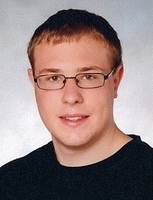
\includegraphics[width=0.25\textwidth]{./04_Projektmanagement/fig/stefanhaefliger.jpg}	&		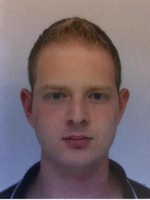
\includegraphics[width=0.25\textwidth]{./04_Projektmanagement/fig/joelmeloni.jpg} 
	\\
	\textbf{Stefan Häfliger} & 	
	\textbf{Joël Meloni}
	\\
	Beladen und Entladen &
	Chassis und Lenkung
\end{tabular}
\end{table}

\large
\textbf{Elektrotechnik}
\begin{table}[H]
\begin{tabular}{p{0.3\textwidth}p{0.3\textwidth}}	
	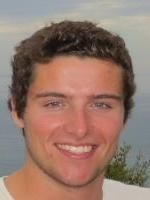
\includegraphics[width=0.25\textwidth]{./04_Projektmanagement/fig/silvanritz.jpg}	&			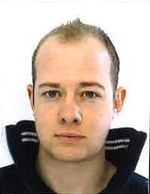
\includegraphics[width=0.27\textwidth]{./04_Projektmanagement/fig/larswalther.jpg} 
	\\
	\textbf{Silvan Ritz} & 	
	\textbf{Lars Walther}
	\\
	Servos, Sensoren und Freescale-Board &
	Energieversorgung und Antrieb
\end{tabular}
\end{table}

\newpage
\large
\textbf{Informatik}
\begin{table}[H]
\begin{tabular}{p{0.3\textwidth}p{0.3\textwidth}p{0.3\textwidth}}	
	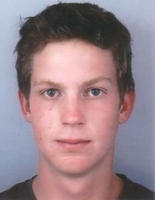
\includegraphics[width=0.26\textwidth]{./04_Projektmanagement/fig/patriziobrantschen.jpg}	&	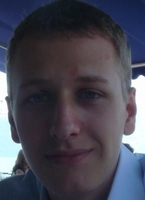
\includegraphics[width=0.24\textwidth]{./04_Projektmanagement/fig/adrianwuersch.jpg} &
	
\includegraphics[width=0.25\textwidth]{./04_Projektmanagement/fig/tobiaskreienbuehl.jpg} 
	\\
	\textbf{Patrizio Brantschen} & 	
	\textbf{Adrian Würsch} &
	\textbf{Tobias Kreienbühl}
	\\
	Objekterkennung und Rechtsvortritt &
	Schnittstellen und Dokumentation &
	Fahrbahnerkennung und Mini-Computer
\end{tabular}
\end{table}
\normalsize








% !TEX root = Dokumentation.tex
\subsection{Zeitplanung}



% !TEX root = Dokumentation.tex
\subsection{Risikomanagement}
Die Risiken, die während der Projektdurchführung entstehen könnten, sind im Folgenden aufgelistet. Um zu wissen, wie hoch ein Risiko eingeschätzt werden muss wurde eine Grafik erstellt. Zu jedem Risiko sind auch Massnhamen aufgelistet, welche im Eintrittsfall unternommen werden können. \\

\begin{figure}[H]%Position festigen
\centering
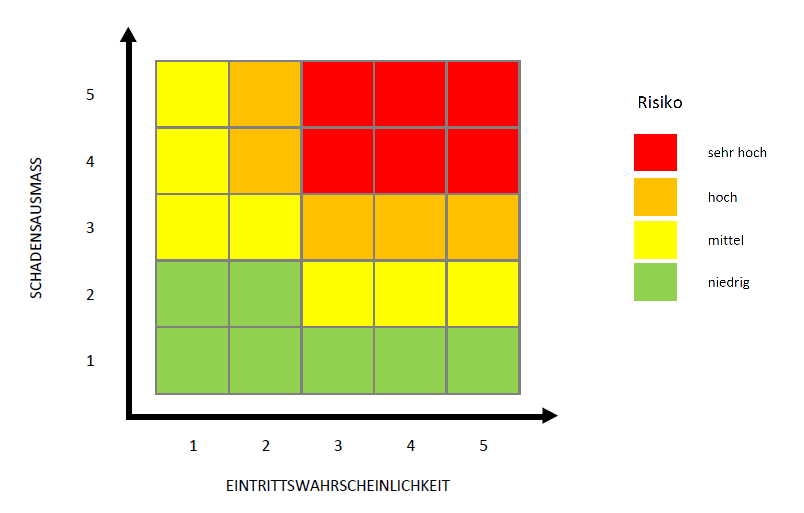
\includegraphics[width=0.8\textwidth]{Images/risikomatrix.png}
\caption{Risikomatrix}
\label{fig:Risikomatrix}
\end{figure}

\subsubsection{Risiken im Team}
\begin{table}[H]
\begin{tabular}{|p{0.3\textwidth}|p{0.2\textwidth}|p{0.2\textwidth}|p{0.2\textwidth}|}\hline
	
	\textbf{Risiko}	& 	\textbf{Wahrscheinlichkeit} & \textbf{Schadensausmass}  & \textbf{Massnahmen} \\\hline
	

	Mitglied verlässt das Team	&	1	&	4	&	Neuverteilung der Arbeiten \\\hline
	Unzuverlässigkeit eines Teammitglieds	&	2	&	3-4	&	 Absprache im Team, um eine Lösung zu finden  \\\hline
	Unstimmigkeiten unter den Teammitgliedern	& 	3	&	4	& Absprache im Team, um eine Lösung zu finden, evtl. auch Rat von Supervisor einholen.  \\\hline
	Mitglied überlastet	&	4	&	3	&	Neuverteilung der Arbeiten \\\hline
	Kommunikations-probleme	&	4	&	3	&	verbessert Absprachen, Frequenz der Sitzungen erhöhen \\\hline
	Fehlende fachliche Kompetenz eines Mitglieds	&	2	&	2	&	Neuverteilung der Arbeiten \\\hline
	Fehlende soziale Kompetenz eines Mitglieds	&	1	&	3	&	Absprache im Team, um eine Lösung zu finden \\\hline
\end{tabular}\\
\end{table}

\subsubsection{Risiken Projektmanagement}
\begin{table}[H]
\begin{tabular}{|p{0.3\textwidth}|p{0.2\textwidth}|p{0.2\textwidth}|p{0.2\textwidth}|}\hline
	
	\textbf{Risiko}	& 	\textbf{Wahrscheinlichkeit} & \textbf{Schadensausmass}  & \textbf{Massnahmen} \\\hline
		Missverständnisse bei den Anforderungen	&	3-4	&	3	& Absprache mit Supervisor  \\\hline
	Ineffizientes Arbeiten	&	3-4	&	2-3	& Neuorganisierung der Vorgehensweise  \\\hline
	
	Überschreitung des Budgets	&	1	&	4	& Absprache mit Supervisor  \\\hline
\end{tabular}\\
\end{table}

\subsubsection{Risiken bei der Realisierung}
\begin{table}[H]
\begin{tabular}{|p{0.3\textwidth}|p{0.2\textwidth}|p{0.2\textwidth}|p{0.2\textwidth}|}\hline
	
	\textbf{Risiko}	& 	\textbf{Wahrscheinlichkeit} & \textbf{Schadensausmass}  & \textbf{Massnahmen} \\\hline
	
	Idee funktioniert nicht wie gewünscht	&	2	&	4 & neue Ideenfindung, Rat einholen  \\\hline
	Eingekaufte Komponente erfüllt Anforderung nicht	&	2	&	5	& andere Komponente einkaufen  \\\hline
		Projekt-anforderungen sind nicht erfüllt	&	1	&	5	&  Anpassungen planen \\\hline
\end{tabular}\\
\end{table}

\subsubsection{Andere Risiken}
\begin{table}[H]
\begin{tabular}{|p{0.3\textwidth}|p{0.2\textwidth}|p{0.2\textwidth}|p{0.2\textwidth}|}\hline
	
	\textbf{Risiko}	& 	\textbf{Wahrscheinlichkeit} & \textbf{Schadensausmass}  & \textbf{Massnahmen} \\\hline
	
	Lange Lieferzeiten bei Bestellungen	&	3	&	2	& andere Arbeiten aufnehmen, früher bestellen  \\\hline
	Github fällt aus	&	1	&	4	& Lokal weiterarbeiten  \\\hline
\end{tabular}\\
\end{table}


% !TEX root = Dokumentation.tex
\subsection{Budgetplanung}

% !TEX root = Dokumentation.tex
\subsection{Projektunterstützung}
Während der Durchführung des Projekts soll der administrative Aufwand möglichst klein gehalten werden können. Weiter sollen alle Projektmitglieder gleichzeitig an der Software weiterentwickeln oder an der Dokumentation weiterschreiben können. Darum wird auf diverse Software-Produkte und -Systeme zurückgegriffen, die sich in der Praxis bewährt haben.
%
\subsubsection{Software}
\begin{table}[H]
\begin{tabular}{|p{0.3\textwidth}|p{0.64\textwidth}|}\hline
%	
Kommunikation	&	E-Mail, Whatsapp \\\hline
Dokumenterstellung & LaTeX\\\hline
Versionsverwaltungssoftware & Git \\\hline
Filehosting-Dienst & GitHub \\\hline
CAD-Software & NX\\\hline
Entwicklungsumgebung	& Eclipse, Kinetis Design Studio \\\hline
%
\end{tabular}
\end{table}
LaTeX ermöglicht es, die gesamte Dokumentation in mehrere Teildokumente zu unterteilen. All diese Dokumente sind in GitHub eingecheckt. Somit wird sichergestellt, dass mehrere Teammitglieder zur selben Zeit an der Dokumentation arbeiten können und dabei möglichst wenig Konflikte entstehen. Weiter wird auf dem selben Git-Repository auch der Quellcode der Software abgelegt. \\
\subsubsection{Aufgabenverteilung}
Um die Aufgabenverteilung festzuhalten wurde ein Scrum-Board erstellt. Darauf sind alle Team-Mitglieder aufgelistet. Zudem sind, wie bei Scrum üblich, die drei Zustände \glqq ToDo\grqq, \glqq Doing\grqq \ und \glqq Done\grqq \ definiert.
\begin{figure}[H]%Position festigen
\centering
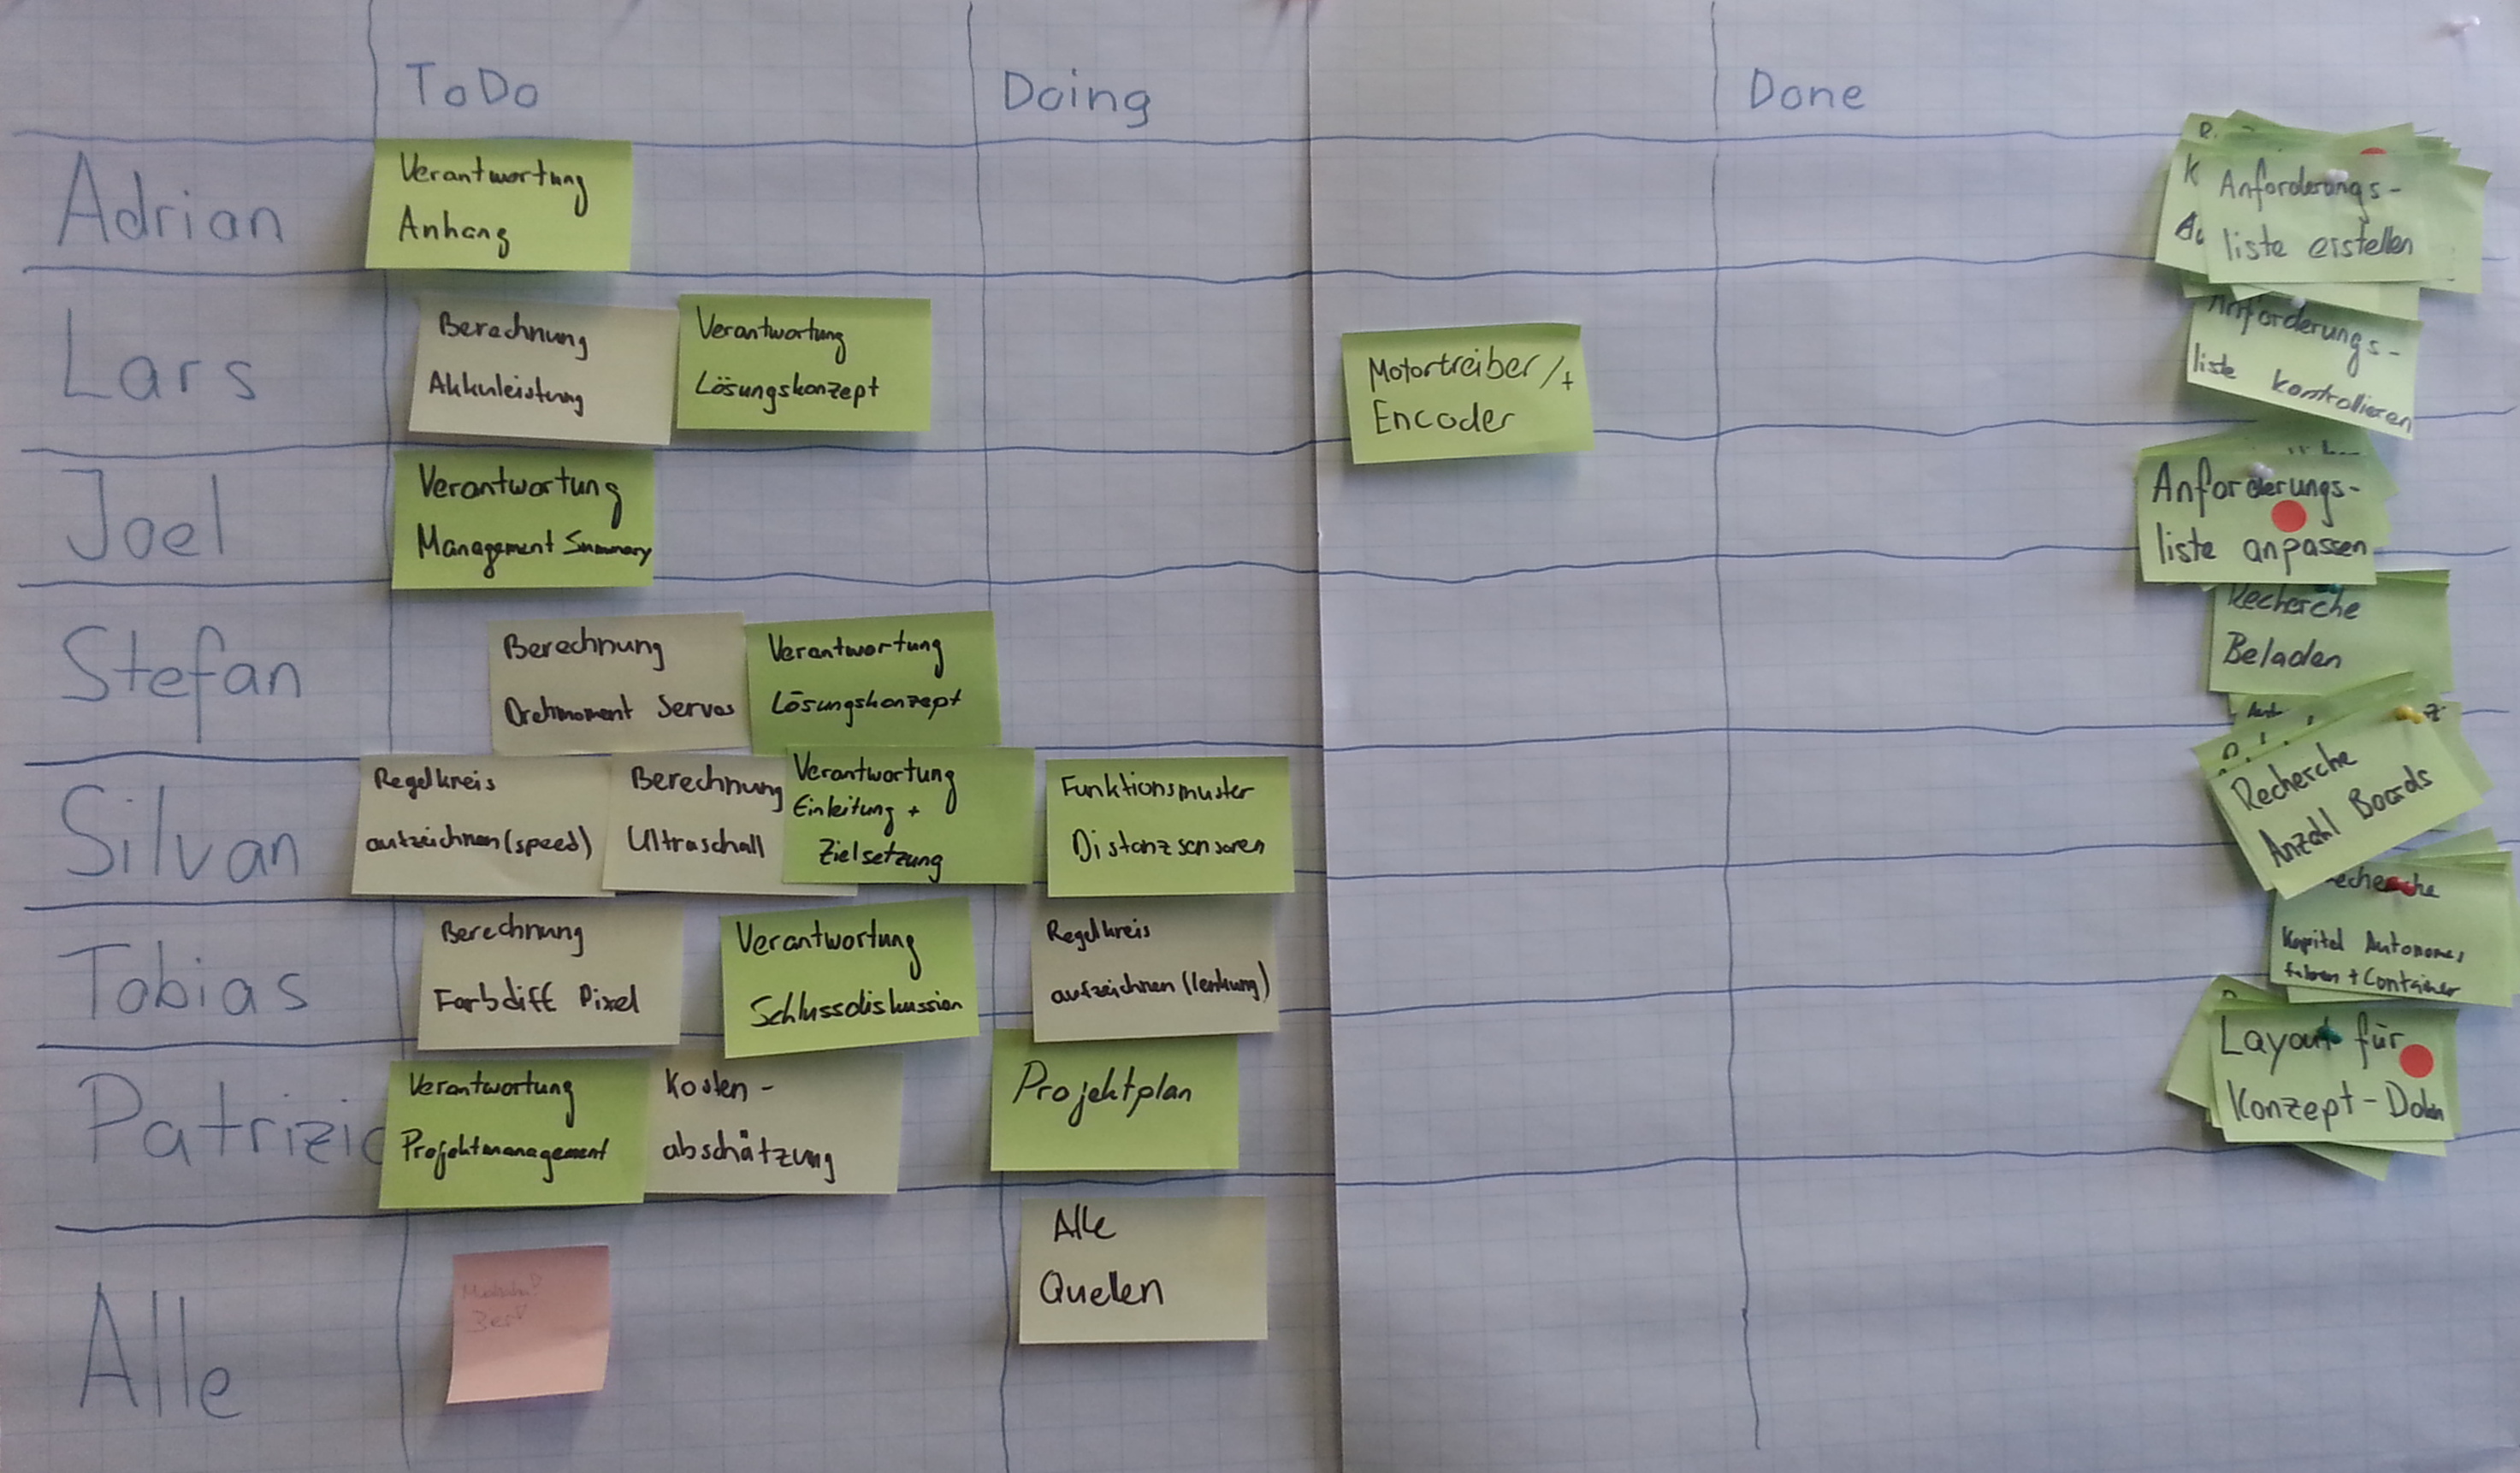
\includegraphics[width=0.8\textwidth]{04_Projektmanagement/fig/scrumBoard.jpg}
\caption{Scrum-Board}
\label{fig:scrumBoard}
\end{figure}
% !TEX root = Dokumentation.tex
\newpage
\section{Bedienungsanleitung}

% !TEX root = Dokumentation.tex
\subsection{Vorbereitung des Fahrzeuges}
\begin{itemize}
\item Überprüfen der korrekten Akkuspannungen
\item Stecker mit Anschlüssen verbinden
\item Drähte korrekt verstauen um Blockierungen zu verhindern 
\end{itemize}

% !TEX root = Dokumentation.tex
\subsection{Starten des Fahrzeuges}
\begin{itemize}
\item Warten bis Raspberry Pi augestartet ist
\item Mit WLAN verbinden, sobald es ersichtlich ist
\item Eine SSH-Verbindung zum Raspberry Pi aufbauen: ssh pi@10.0.0.1
\item Minicom starten
\item Die Datei ./StartGueselStar im Home-Verzeichnis ausführen
\end{itemize}


% !TEX root = Dokumentation.tex
\subsection{Fehlerbehebung}



% !TEX root = Dokumentation.tex
\section{Schlussdiskussion}

% !TEX root = Dokumentation.tex
\subsection{Entwicklungskosten und -aufwand}
% !TEX root = Dokumentation.tex
\subsection{Lessons Learned}
Bei einer Projektarbeit mit interdisziplinärer Zusammenarbeit ist es wichtig, sich früh auf einen Konsens zu einigen.
Für das Team war es wichtig, sich immer gemeinsam zu entscheiden und so immer alle möglichen Auswirkungen im Blick zu haben.
Durch das Definieren von Schnittstellen bereits zu Begin, konnten viele Missverständnisse bereits in der Planungsphase bereinigt werden.
\\[0.2cm]
Gewisse OpenSource Lösungen bieten zwar eine breite und solide Palette von Funktionen an, sind aber schlecht auf eine spezifische Aufgabe skalierbar.
Ein motivierteres Mitglied der Gruppe hat sich die Zeit genommen und mit vertieftem mathematischen Wissen einen sehr effizienten Algorithmus entwickelt.
Dieser schlanke, auf die Aufgabe zugeschnittene Algorithmus ermöglicht das Auswerten des Bildmaterials nahezu in Echtzeit.
\\[0.2cm]
Einige Mitglieder des Teams haben ein persönliches Engagement für Lego Bauteile. Dies machte sich nützlich, um ein erstes Fahrzeug zu visualisieren.
Mit diesem provisorischen Lego-Fahrzeug konnte die Strecke abgefahren werden. So wurden einige Problemstellen aufgedeckt, welche vorher nicht beachtet wurden. Durch diese simple Tat konnte die zukünftige Umsetzung massiv beeinflusst werden.
\\[0.2cm]
Zu Begin setzte sich das Team zusammen und diskutierte über alle benötigten Funktionen und Bauteile.
Dies ermöglichte den Maschinenbauern ein Fahrzeug zu modellieren, welches genug Platz bietet und innerhalb der Grössenordnung bleibt.
Durch dieses Vorgehen ist frühzeitig sichergestellt, dass alle Funktionalitäten abgedeckt sind und zeitig Fertigungsteile bestellt werden können.
\\[0.2cm]
Um eine Gruppe zu bilden und erfolgreich zu führen braucht es zwingend zwei Dinge.
Die gleichen Ziele und die gleichen Regeln für alle Mitglieder.
Doch wo es Regeln gibt, wird es auch Verstösse geben. Deshalb hat sich das Team früh auf eine adäquate Strafe geeinigt.
Kommt jemand zu spät oder gar nicht, so soll derjenige das Team mit Getränken versorgen.
So ist sichergestellt, dass genügend Motivation vorhanden ist und auch die anderen bei solch einem Missgeschick profitieren.
% !TEX root = Dokumentation.tex
\subsection{Offene Punkte}
% !TEX root = Dokumentation.tex
\subsection{Risiken}
% !TEX root = Dokumentation.tex
\subsection{Ausblick PREN2}

Ende PREN1 wurde ein Lösungskonzept ausgewählt und detailliert ausgearbeitet.
Die Aufgaben sind klar verteilt und das Team versteht sich gut. PREN2 geht nun nahtlos weiter und setzt die Planung in die Realität um.
Besonders ins Auge sticht die komplexe Navigation auf dem Spielfeld und das Zusammenspiel der vielen Sensoren.
Das Team freut sich auf die neuen Herausforderungen, die umso grösser sind, da ein Mitglied die Gruppe verlässt.


\end{document}